\documentclass[hyperref=colorlinks]{beamer}
\mode<presentation>
\usetheme{iclpt}
\setbeamertemplate{navigation symbols}{}
\setbeamertemplate{headline}{
\begin{beamercolorbox}[leftskip=.2cm,rightskip=.2cm,topskip=.2cm,ht=1.1cm,dp=0.1cm,wd=\textwidth]{institute in head/foot}
  
\includegraphics[height=1cm]{icl.pdf}
  \hfill
  
\includegraphics[height=1cm]{../Pics/CMS-Color.pdf}
\end{beamercolorbox}
}
\setbeamertemplate{footline}{
\begin{beamercolorbox}[ht=.55cm,dp=0.4cm,wd=\textwidth,leftskip=.3cm]{author in head/foot}%
  \begin{minipage}[c]{5cm}%
    \usebeamerfont{author in head/foot}
    \insertshortauthor 
    \insertshorttitle
    \end{minipage}\hfill%
  \insertframenumber{} / \pageref{lastframe}
  \hfill
  \begin{minipage}{6cm}
    \hfill
  \end{minipage}
\end{beamercolorbox}%
}

\usepackage{color}
\usepackage{tabularx,colortbl}
\usepackage{graphicx}
\usepackage{pdfpages}
\usepackage{feynmp}
\DeclareGraphicsRule{*}{mps}{*}{}

\title{\vspace{-0.2cm} Higgs to Invisible Analyses at CMS}
\subtitle{PAS-HIG-13-013, HIG-13-030 \vspace{-0.7cm}}
\author[P. Dunne]{R. Aggleton, C. Asawatangtrakuldee, J. Brooke, O. Buchmueller D. Colling, G. Davies \underline{P. Dunne}, S. Kumar, Q. Li,  A. Magnan, K. Mazumdar, A. Nikitenko, J. Pela, P. Srimanobhas}%!!FIX AUTHOR LIST AND TITLE GRAPHIC GO FROM COMB OR HIGGS EXO PRESENTATION
\titlegraphic{
  \vspace{-0.7cm}
\begin{fmfgraph*}(100,70)
        \fmfleft{i1,i2}
        \fmfright{o1,o2,o3}
        \fmf{fermion}{i1,v1,o1}
        \fmf{fermion}{i2,v2,o3}
        \fmf{phantom,tension=4/5}{v1,v2}
        \fmffreeze
        \fmf{photon,label=$W,,Z$}{v1,v3}
        \fmf{photon,label=$W,,Z$}{v2,v3}
        \fmf{dashes}{v3,o2}
        \fmflabel{$q$}{i1}
        \fmflabel{$q$}{i2}
        \fmflabel{$q$}{o1}
        \fmflabel{$q$}{o3}
        \fmflabel{$H$}{o2}
      \end{fmfgraph*}
}
\date{}
\begin{document}
\begin{fmffile}{feynmandiags}

%TITLE PAGE
\section{Title}
\begin{frame}
  \titlepage

 \end{frame}

 %OUTLINE
 \begin{frame} %!!UPDATE
   \frametitle{Introduction}
   \begin{columns}
     \column{.6\textwidth}
     \begin{itemize}
     \item Searching for VBF produced Higgs decaying to invisible final state
     \item Visible decays constrain invisible BF to less than 64\% at 95\% C.L. (assumes standard model width)
     \item Many theoretical possibilities for BSM invisible final states:
     \item[-] $H\rightarrow 2 LSPs$ (SUSY)
     \item[-] $H\rightarrow$ dark matter (Extra Dimensions)
     \item[-] etc.
     \end{itemize}
     \column{.4\textwidth}
     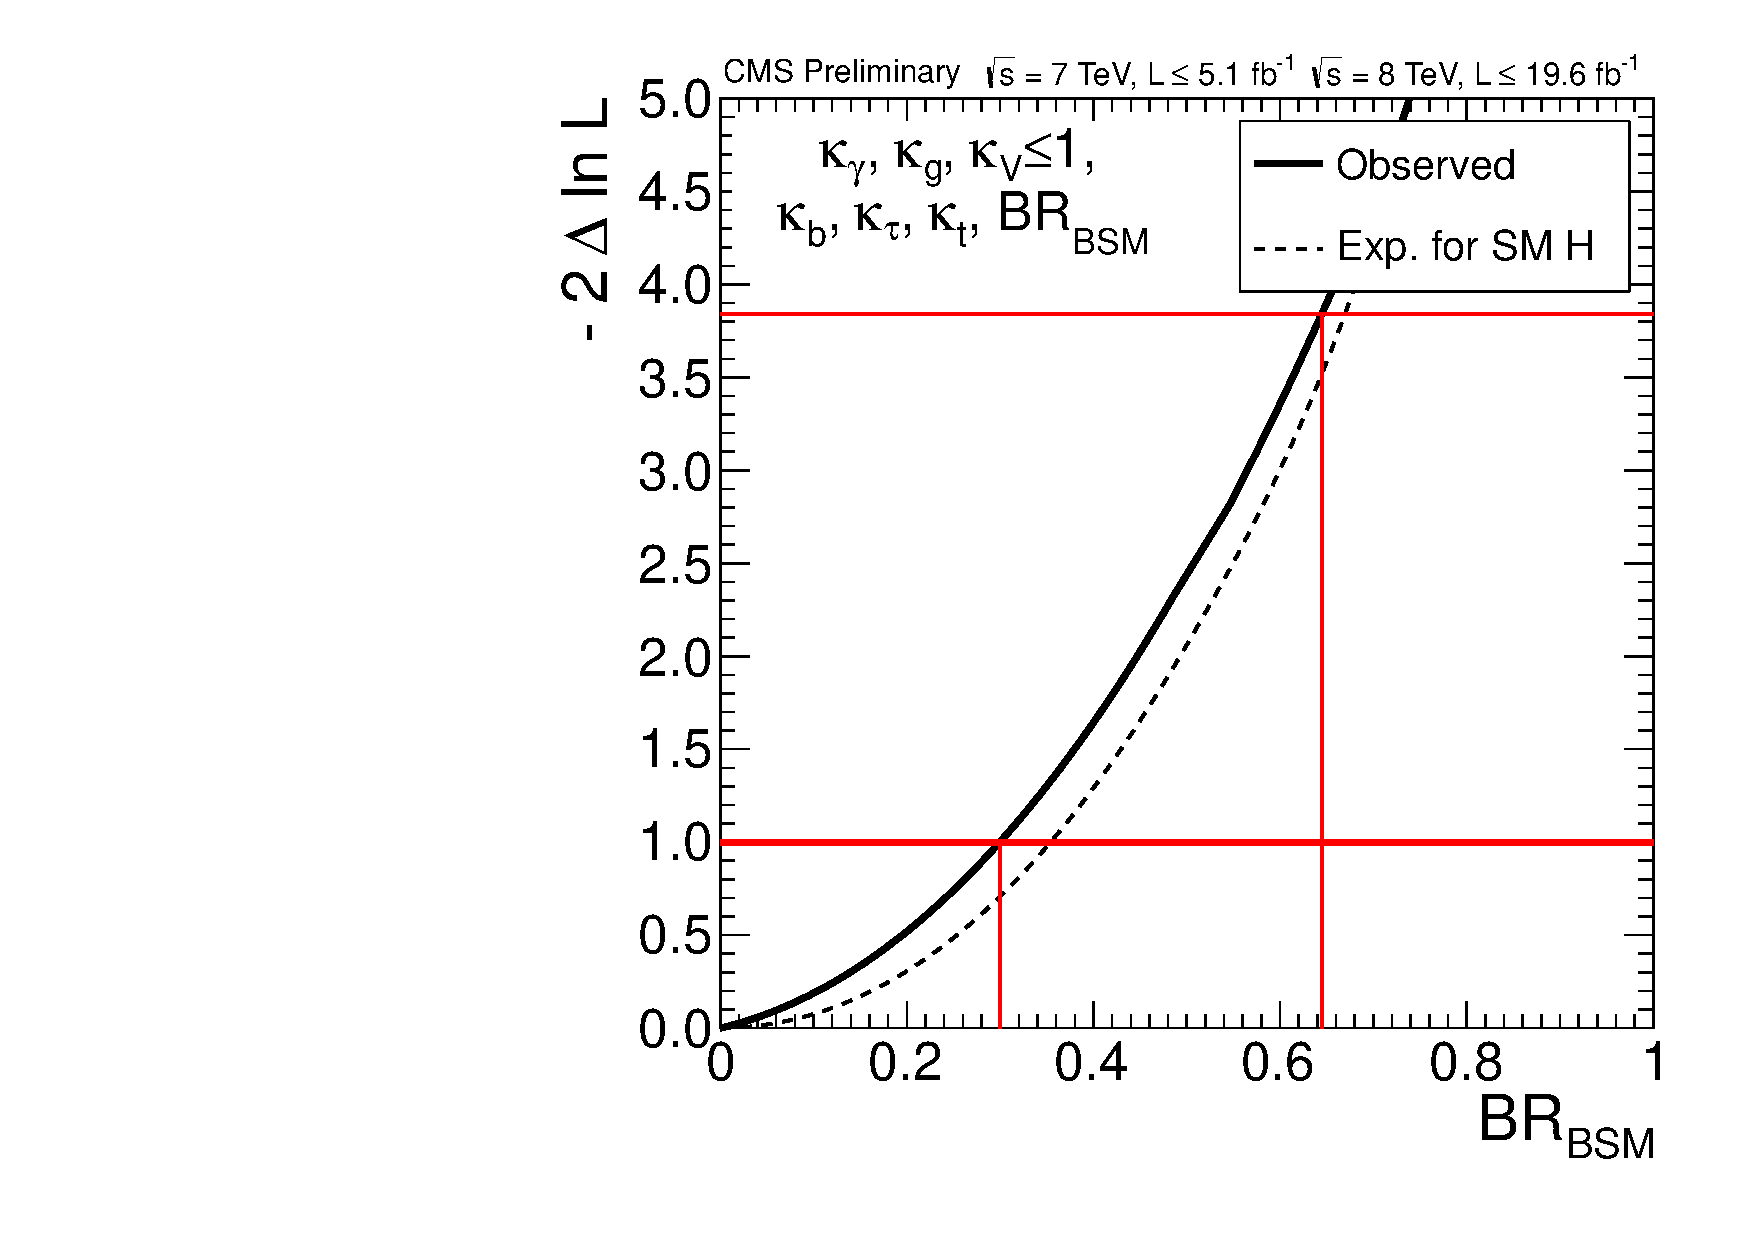
\includegraphics[width=\textwidth]{TalkPics/invbr.pdf}
   \end{columns}
 \end{frame}

 %OVERALL STRATEGY
 \begin{frame}%!!MAKE MORE GENERAL TO ALL THREE ANALYSES
   \frametitle{Measurement Strategy}
   \begin{columns}
     \column{.5\textwidth}
     
     \scriptsize
     \begin{block}{\scriptsize General Strategy}
       \begin{itemize}
       \item Clean data from pileup and mismeasured MET
       \item Use hard cuts to restrict backgrounds
       \item Remaining background estimation must be data driven as hard cuts make MC unreliable
       \end{itemize}
     \end{block}

     \vspace{.25cm}

     \begin{figure}
     \begin{fmfgraph*}(100,70)
       \fmftop{i1,m1,o1}
       \fmfbottom{i2,o2}
       \fmf{fermion}{v1,o2}
       \fmf{fermion}{v1,i2}
       \fmf{dashes,label=$H$}{v1,m1}
       \fmflabel{$jet$}{i2}
       \fmflabel{$jet$}{o2}
       \fmflabel{$MET$}{m1}
     \end{fmfgraph*}
     \end{figure}



     \column{.5\textwidth}
     \centering
     \begin{block}{\scriptsize Select VBF Topology}
       \scriptsize
       \begin{itemize}
       \item 2 jets with a large $\eta$ separation
       \item Nothing in the gap between the jets
       \item Need dedicated VBF trigger
       \end{itemize}
     \end{block}
     
     \begin{block}{\scriptsize Cuts}
       \scriptsize
       \begin{itemize}
       \item Require 2 jets in all regions:
       \item[-] Both jets must pass loose PUJetID
       \item[-] $p_{T} > 50 GeV$,  $|\eta| < 4.7$
       \item[-] $|\Delta\eta|>4.2$ , $\eta_{j_{1}}*\eta_{j{_2}}<0$
       \item[-] $m_{jj} > 1100 GeV$
       \item Veto events with jets with $p_{T}>30$GeV between the tag jets unless stated otherwise (CJV)
      \end{itemize}
     \end{block}

     
  \end{columns}
\end{frame}

%!!DO A SECTION ON EACH ANALYSIS

\begin{frame}
  \frametitle{Backgrounds Overview}
  \begin{columns}
    \column{.6\textwidth}
    \vspace{-0.3cm}
    \begin{block}{\scriptsize Main backgrounds:}
      \scriptsize
      \begin{itemize}
      \item $W$ + jets where lepton is missed
      \item[-] {\color{red}AM+Patrick cross check}
      \item $Z\rightarrow\nu\nu$ + jets
      \item QCD: {\color{red}Sasha}
      \end{itemize}
    \end{block}
    \vspace{-0.3cm}
    \begin{block}{\scriptsize Data driven $W/Z$ + jets estimation:}
      \scriptsize
      \begin{itemize}
      \item Pick $W/Z$ dominated control region in same trigger sample with same VBF selection
      \item[-] For muons recalculate MET after removing leptons from $W$ \& $Z$ to mimic $W$ with missed muon/$Z\rightarrow\nu\nu$
      \item Check data/MC shape agreement in control regions
      \item Assume MC signal/control ratio is the same as that in data
      \end{itemize}
    \end{block}
    \column{.05\textwidth}
    \column{.35\textwidth}
    %WJETS
    \begin{fmfgraph*}(75,60)
      \fmftop{i1,m1,m2,o1}
      \fmfbottom{i2,o2}
      \fmf{fermion,label=$e/\mu/\tau$,label.side=left}{v2,m1}
      \fmf{fermion,label=$\nu$,label.side=right}{v2,m2}
      \fmf{photon,tension=7/5,label=$W$}{v1,v2}
      \fmf{fermion}{v1,i2}
      \fmf{fermion}{v1,o2}
      \fmflabel{$jet$}{i2}
      \fmflabel{$jet$}{o2}
    \end{fmfgraph*}
    \vspace{0.2cm}
    %ZJETS
    \begin{fmfgraph*}(75,50)
      \fmftop{i1,m1,m2,o1}
      \fmfbottom{i2,o2}
      \fmf{fermion}{v1,i2}
      \fmf{fermion}{v1,o2}
      \fmf{photon,tension=7/5,label=$Z$}{v1,v2}
      \fmf{fermion,label=$\nu$,label.side=left}{v2,m1}
      \fmf{fermion,label=$\nu$,label.side=right}{v2,m2}
      \fmflabel{$jet$}{i2}
      \fmflabel{$jet$}{o2}
    \end{fmfgraph*}
    
    %QCD
    \begin{fmfgraph*}(75,60)
      \fmftop{i1,m1,m2,m3,m4,o1}
      \fmfbottom{i2,o2}
      \fmf{fermion,tension=4}{v1,i2}
      \fmf{fermion,tension=4}{v1,o2}
      \fmf{fermion,label=$jets$,label.side=left}{v1,m1}
      \fmf{fermion}{v1,m2}
      \fmf{fermion}{v1,m3}
      \fmf{fermion}{v1,m4}
      \fmflabel{$jet$}{i2}
      \fmflabel{$jet$}{o2}
    \end{fmfgraph*}
  \end{columns}
\end{frame}

%TRIGGER AND DATASETS
\begin{frame}
  \frametitle{Datasets and Trigger}
  \begin{columns}
    \column{.5\textwidth}
    \vspace{-0.2cm}
    \begin{block}{\scriptsize Datasets:}
      \scriptsize
      \begin{itemize}
      \item 8 TeV MET datasets
      \item[-] Total of 19.6 $fb^{-1}$
      \item MET filters are used to cut out events with mismeasured MET
      \end{itemize}
    \end{block}
    \vspace{-0.3cm}
    \begin{block}{\scriptsize Trigger:}
      \scriptsize
      \begin{itemize}  
      \item HLT\_DiPFJet40\_PFMET noMu65\_MJJ800VBF\_AllJets
      \item[-] VBF means $|\Delta \eta_{j_{1}j_{2}}| > 3.5 $
      \item {\color{red} IC heavily involved in design of the trigger}
      \end{itemize}
    \end{block}
    \column{.5\textwidth}
    \centering
    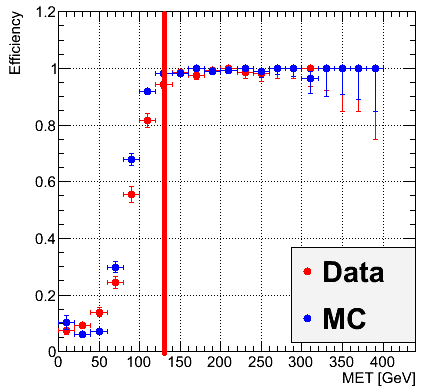
\includegraphics[height=.45\textheight]{TalkPics/METtrig.png}
    
    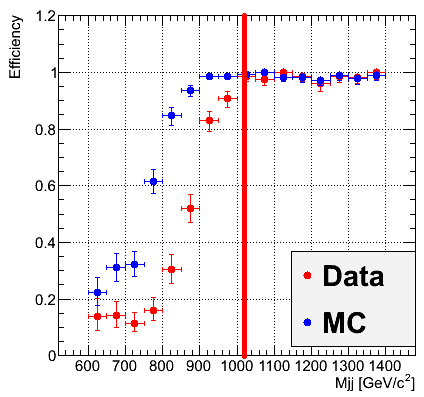
\includegraphics[height=.45\textheight]{TalkPics/Mjjtrig.png}
  \end{columns}
\end{frame}

%SIGNAL EVENT SELECTION
\begin{frame}
    \frametitle{Signal Event Selection}
  \vspace{-0.2cm}
  \begin{block}{\scriptsize Signal Region Selection:}
    \scriptsize
    \begin{itemize}
    \item PFMET $> 130GeV$, $\Delta\phi_{jj}<1.0$ to reduce QCD
    \item $e/\mu$ veto to reduce $W/Z$+jets
    \end{itemize}
  \end{block}
  \vspace{-0.15cm}
  \begin{columns}
    \column{.5\textwidth}
    \column{.5\textwidth}
    \scriptsize Data MC difference is QCD
  \end{columns}
  \begin{columns}
    \column{.5\textwidth}
    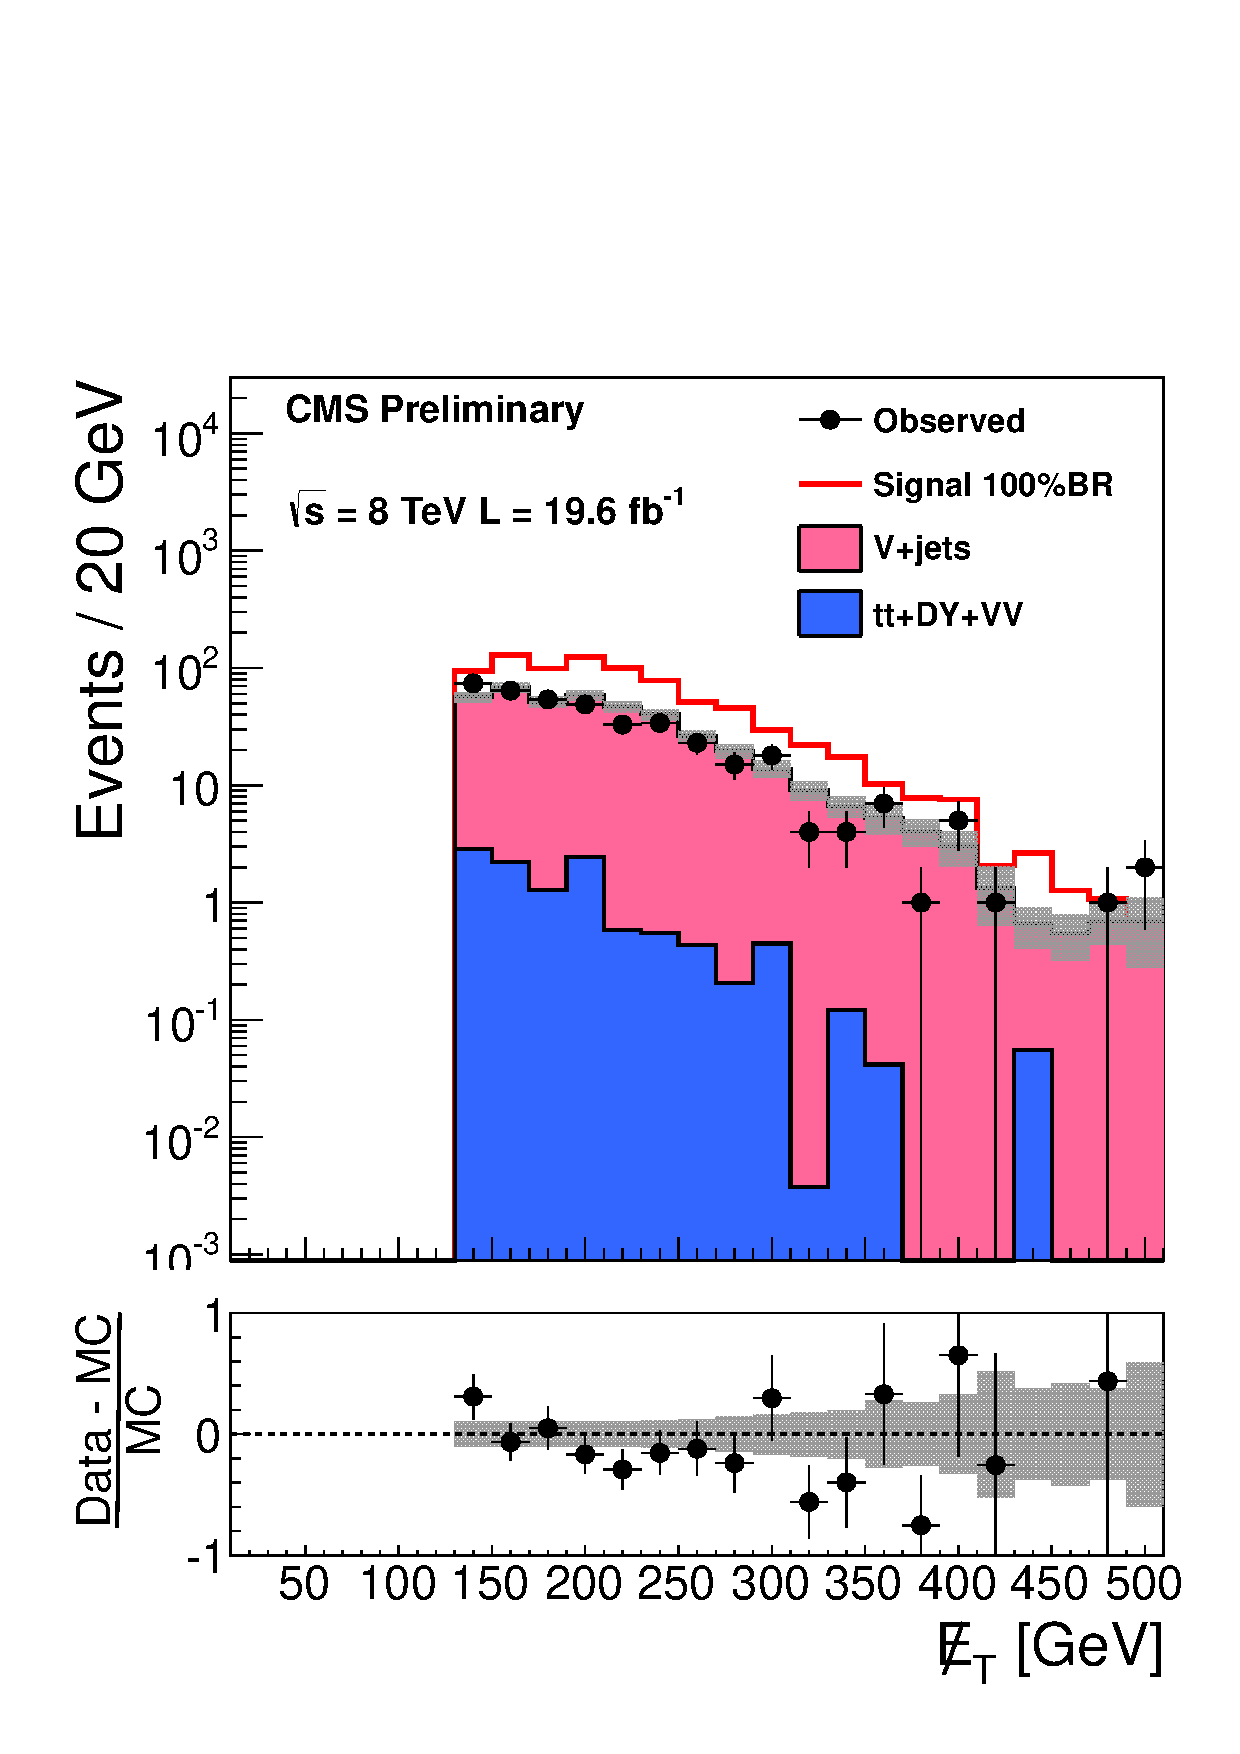
\includegraphics[width=\textwidth,height=.5\textheight]{TalkPics/iccms091013/hMETNM1.pdf}
    \column{.5\textwidth}
    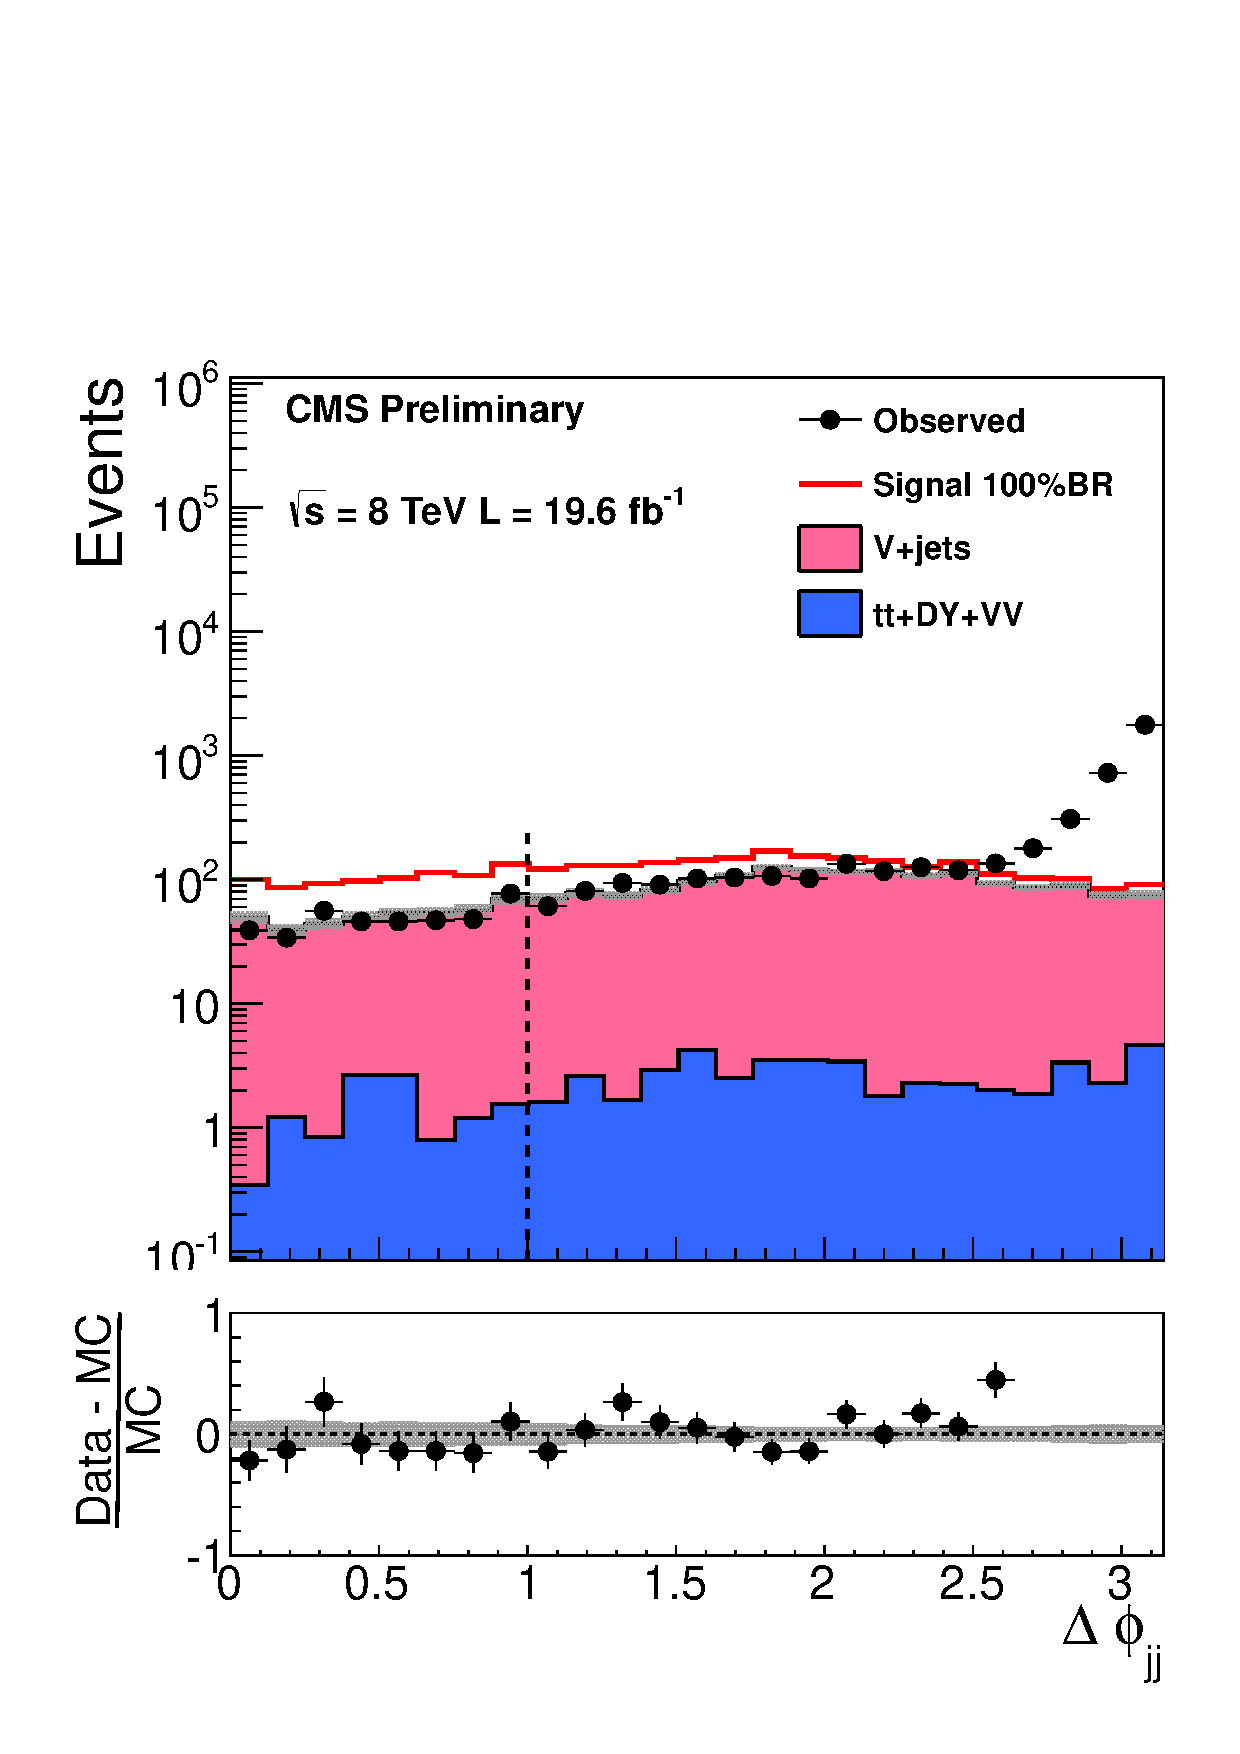
\includegraphics[width=\textwidth,height=.5\textheight]{TalkPics/iccms091013/hDPhiJJNM1.pdf}
  \end{columns}
\tiny
\vspace{-0.1cm}
\end{frame}

%BACKGROUNDS

%Background estimations!
\begin{frame}
  \frametitle{$W$+jets Background Estimation}
  \vspace{-0.4cm}
  \begin{columns}
    \column{.5\textwidth}
    \begin{block}{\scriptsize Background estimation formula:}
      \scriptsize
      \centering
      $N^{S}_{data} (W\rightarrow e/\mu) = (N^{C}_{data}-N^{C}_{bkg})\frac{N^{S}_{MC}}{N^{C}_{MC}}$  
    \end{block}
    \column{.5\textwidth}
    \begin{block}{\scriptsize $W \rightarrow \mu/ e$ Control Region Selection:}
      \scriptsize
      \begin{itemize}
      \item 1 tight muon/electron:
      \item MET $>130 GeV$
      \end{itemize}
    \end{block}
  \end{columns}
  \begin{columns}
    \column{.5\textwidth}
    \centering
    \scriptsize
    $W\rightarrow e\nu$
    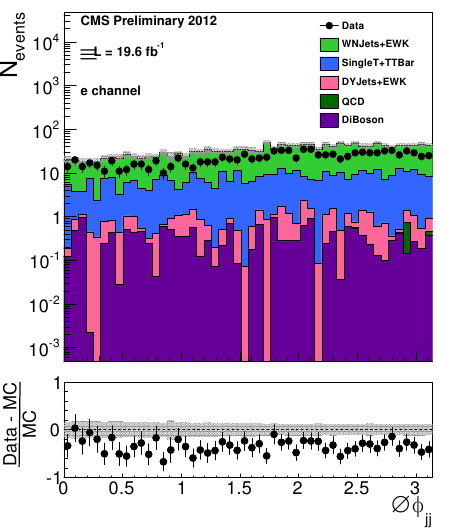
\includegraphics[width=\textwidth,height=.5\textheight]{TalkPics/iccms091013/dphijjwe.png}
    \column{.5\textwidth}
    \centering
    \scriptsize
    $W\rightarrow \mu\nu$
    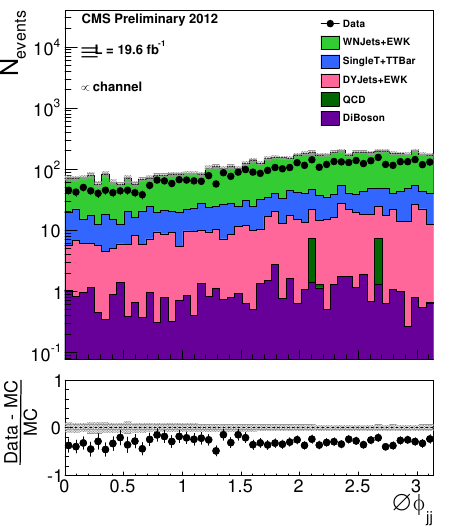
\includegraphics[width=\textwidth,height=.5\textheight]{TalkPics/iccms091013/dphijjwmu.png}
  \end{columns}
  \vspace{-0.2cm}
  
  \begin{columns}
    \column{.5\textwidth}
    \begin{block}{}
      \scriptsize
      \centering
      $N^{S}_{data} =$ $68.2\pm 9.2(stat.)\pm 13.1(syst.)$ events
    \end{block}
    \column{.5\textwidth}
    \begin{block}{}
      \scriptsize
      \centering
      $N^{S}_{data} =$ $67.2\pm 5.0(stat.) \pm 7.5 (syst.)$ events
    \end{block}
  \end{columns}
\end{frame}

\begin{frame}
  \frametitle{$W\rightarrow\tau_{\tiny had}\nu$ Background Estimation}
  \begin{columns}
    \column{.5\textwidth}
    \vspace{-0.3cm}
    \vspace{-0.2cm}
    \begin{block}{\scriptsize Background estimation formula:}
      \scriptsize
      \centering
      $N^{S}_{data} (W\rightarrow \tau\nu) = (N^{C}_{data}-N^{C}_{bkg})\frac{N^{S}_{W\rightarrow\tau\nu MC}}{N^{C}_{W\rightarrow\tau\nu MC}}$  
    \end{block}
    \begin{block}{\scriptsize $W\rightarrow \tau$ Control Region Selection:}
      \scriptsize
      \begin{itemize}
      \item Require signal region criteria except CJV
      \item Require 1 $\tau_{hadronic}$ candidate
      \item[-] No tau veto so this is a subsample of signal region without CJV
      \end{itemize}
    \end{block}
    \vspace{-0.2cm}
    \begin{block}{\scriptsize Result}
      \scriptsize
      \begin{itemize}
      \item $N^{data}_{W\rightarrow\tau\nu} = 54 \pm 16(stat.)\pm18(syst.)$
      \end{itemize}
    \end{block}
    \column{.5\textwidth}
    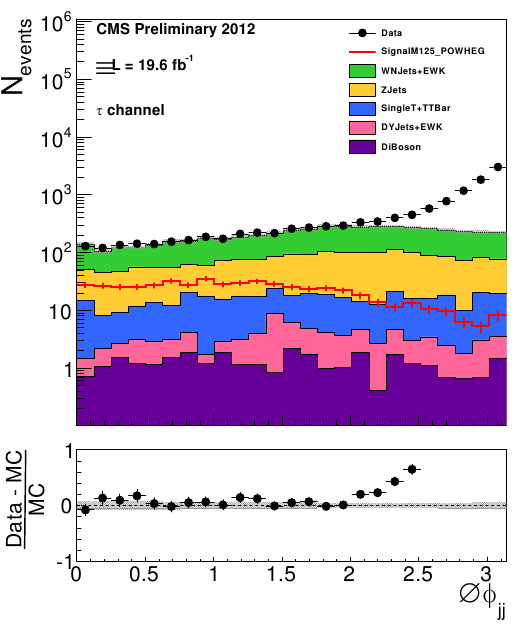
\includegraphics[width=\textwidth]{TalkPics/iccms091013/dphijjwtau.png}

  \end{columns}
\end{frame}


\begin{frame}
  \frametitle{$Z$+jets Background Estimation}
  \begin{block}{\scriptsize Z+jets background estimation formula:}
    \scriptsize 
    \centering
    $N^{S}_{data}(Z\rightarrow\nu\nu)=(N^{C}_{data} - N^{C}_{bkg})\frac{\sigma(Z\rightarrow\nu\nu)}{\sigma(Z/\gamma^{*}\rightarrow\mu\mu)}\frac{\epsilon^{S}_{VBF}/\epsilon^{C}_{VBF}}{\epsilon_{\mu\mu}}$
  \end{block}
  \begin{columns}
    \column{.5\textwidth}
    \begin{block}{\scriptsize $Z\rightarrow\nu\nu$ Control Region Selection:}
      \scriptsize
      \begin{itemize}
      \item Select $Z\rightarrow\mu\mu$ and extrapolate to $Z\rightarrow\nu\nu$
      \item[-] 2 tight muons with $60<M_{\mu\mu}<120$ GeV
      \item[-] MET after $Z$ candidate removed $> 130 GeV$
      \item[-] No additional veto muons/electrons
      \end{itemize}
    \end{block}
    \begin{block}{}
      \centering
      \scriptsize
      $N^{S}_{data}=102\pm30(stat.)\pm 14(syst.)$
    \end{block}
    \column{.05\textwidth}
    \column{.4\textwidth}
    \vspace{-.05cm}

    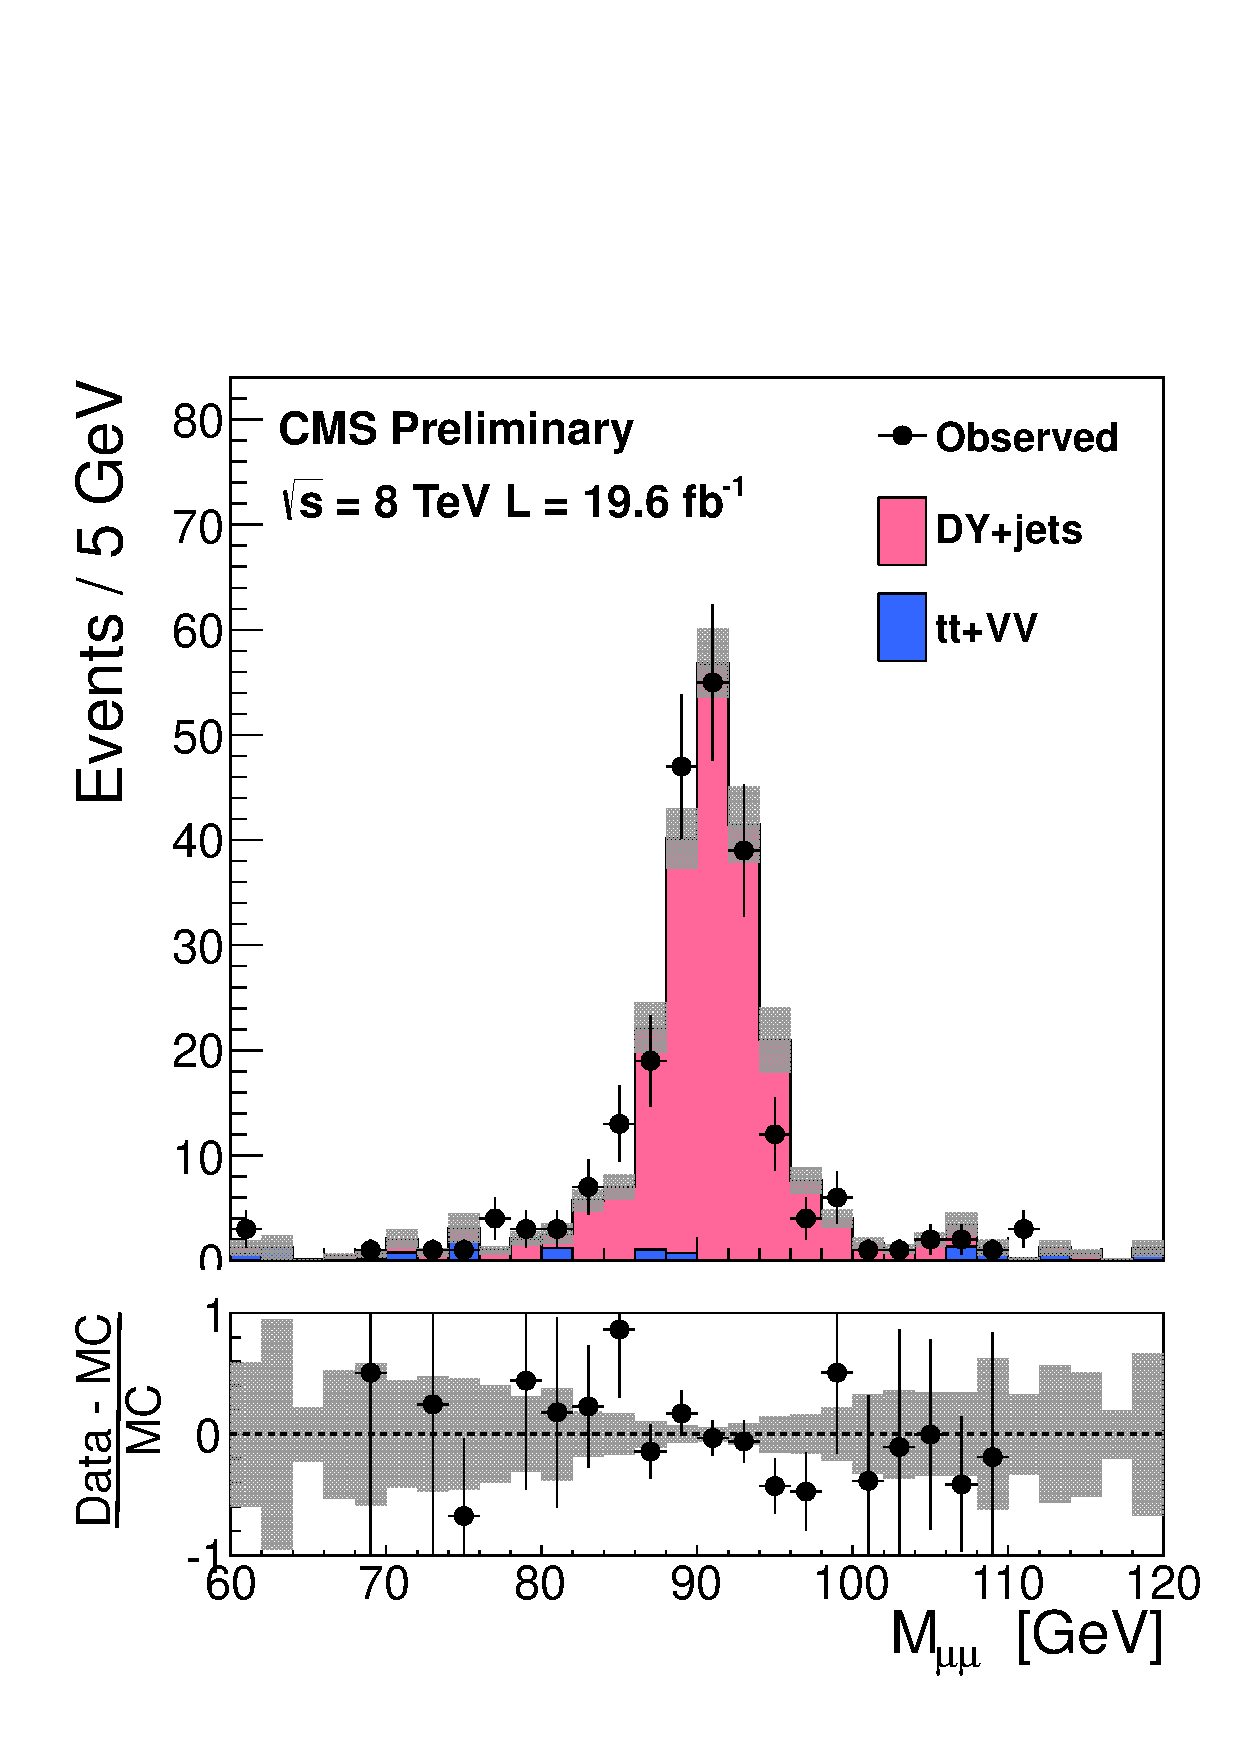
\includegraphics[width=.95\textwidth]{TalkPics/iccms091013/ZCtrlZMass.pdf}
  \end{columns}
\end{frame}

\begin{frame}
  \frametitle{Consistency Tests}
  \begin{columns}
    \column{.5\textwidth}
    \begin{block}{\scriptsize Method}
      \scriptsize
      \begin{itemize}
      \item To check $W/Z$+Jets estimates the $W\rightarrow\mu\nu$ sample is used to predict the other control region yields
      \item The predictions are consistent with the observed yields for all control regions
      \item[-] Some regions with significant QCD contamination show deviations
      \end{itemize}
    \end{block}
    \column{.5\textwidth}
    \centering
    \begin{block}{\scriptsize $W\rightarrow e\nu$ from $W\rightarrow\mu\nu$}
    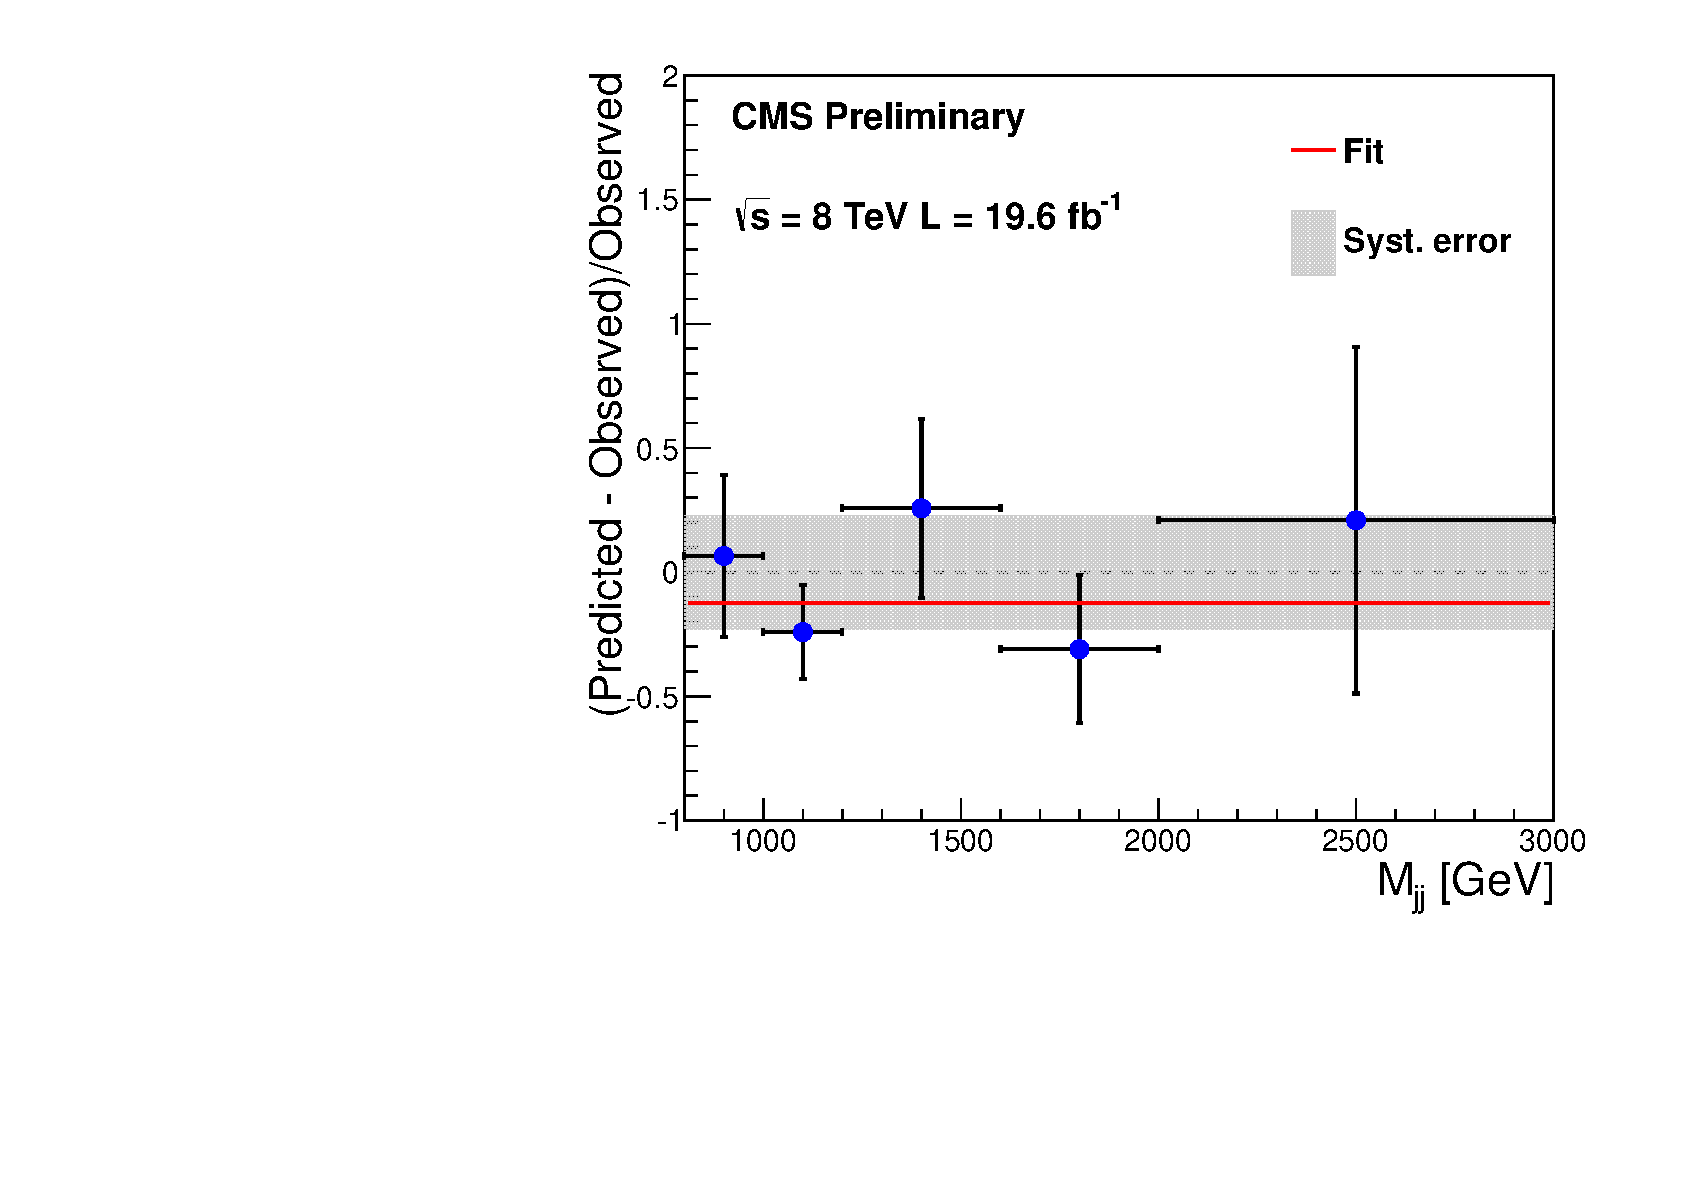
\includegraphics[width=\textwidth]{TalkPics/iccms091013/MJJ_Welnu_frac.pdf}
    \end{block}
  \end{columns}
\end{frame}

%QCD
\begin{frame}
  \frametitle{QCD}
  \begin{columns}
    \column{.5\textwidth}
    \begin{block}{\scriptsize QCD Background Strategy}
      \scriptsize
      \begin{itemize}
      \item V. low MC statistics
      \item[1)] Reduce background with cuts
      \item[2)] Estimate using data driven ABCD method in MET and CJV
      \item[3)] Cross-check using ABCD method in MET and $\Delta\phi_{jj}$
            \end{itemize}
    \end{block}
    \begin{block}{\scriptsize QCD ABCD method:}
      \scriptsize
      \begin{itemize}
      \item Choose 4 regions:
      \end{itemize}
      \begin{tabular}{|l|c|c|}
        \hline
        & Fail MET & Pass MET \\
        \hline
        Fail CJV & A & B \\
        \hline
        Pass CJV & C & D (signal) \\
        \hline
      \end{tabular}
      \begin{itemize}
      \item $N_{D}=N_{B}N_{C}/N_{A}$
      \end{itemize}
    \end{block}
    \column{.5\textwidth}
    \begin{block}{}
      \scriptsize
      \begin{itemize}
      \item $N_{QCD}=36.8\pm5.6(stat.)\pm30.6{syst.}$
      \end{itemize}
    \end{block}

    \vspace{.5cm}

    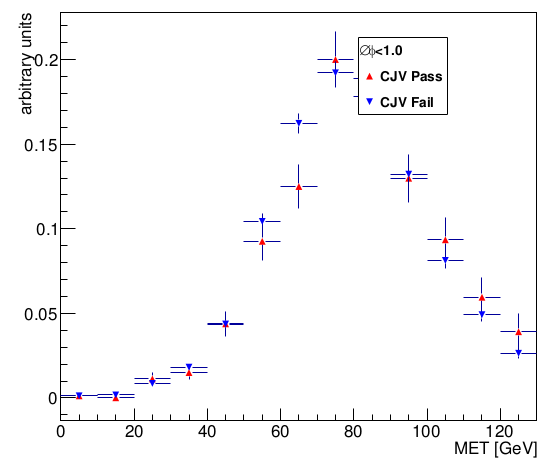
\includegraphics[width=\textwidth,height=.6\textheight]{TalkPics/iccms091013/qcdmet.png}
  \end{columns}
\end{frame}

%!!MAKE THIS PART MORE GENERAL COMBINATIONS AND CORRELATIONS

\begin{frame}
  \frametitle{Uncertainties}
  \begin{columns}
    \column{.5\textwidth}
    \begin{block}{}
      \scriptsize
      \begin{table}\tiny
        \setlength{\tabcolsep}{3pt}
        \begin{tabular}{|l|c|c|}
          \hline
          Background & Source & Uncertainty \\
          \hline
          $Z\rightarrow\nu\nu$ & Statistics in control region & 29\% \\
          & MC statistics & 14\% \\
          & Theory uncertainty & 20\% \\
          & Jet/MET scale/resolotion & 5\% \\
          \hline
          $W\rightarrow\mu\nu$ & Statistics in control region & 5\% \\
          & MC statistics & 10\% \\
          & Theory uncertainty & 20\% \\
          & Jet/MET scale/resolotion & 4\% \\
          \hline
          $W\rightarrow e\nu$ & Statistics in control region & 10\% \\
          & MC statistics & 10\% \\
          & Theory uncertainty & 20\% \\
          & Jet/MET scale/resolotion & $^{+5}_{-11}$\% \\
          \hline
          $W\rightarrow\tau\nu$ & Statistics in control region & 30\% \\
          & MC statistics & 20\% \\
          & Theory uncertainty & 20\% \\
          & Jet/MET scale/resolotion & $^{+16}_{-2}$\% \\
          & Tau ID efficiency & 8\% \\
          & Electron contamination & 5\% \\
          \hline
        \end{tabular}
      \end{table}
      \vspace{-.4cm}
    \end{block}
    
    \column{.5\textwidth}
    \begin{block}{}
       \scriptsize
       \begin{table}\tiny
         \setlength{\tabcolsep}{3pt}
         \begin{tabular}{|l|c|c|}
           \hline
           Background & Source & Uncertainty \\
           \hline
           QCD & Statistics in control region & 2\% \\
           & MC statistics (background) & 2\% \\
           & Jet/MET scale/resolution & $^{+45}_{-75}$\% \\
           & MET shape & 35\% \\
           \hline
           Other & Luminosity & 4\% \\
           backgrounds & MC statistics & 10 \% \\
           & Jet/MET scale/resolution & 28-81\% \\
           & Cross-section uncertainty & 8-20\% \\ 
           \hline
           Signal & MC statistics & 10\% \\
           & Jet/MET scale/resolution & 11\% \\
           & PDF uncertainty & 5\% \\
           & QCD scale uncertainty & 4\% \\
           \hline
         \end{tabular}
       \end{table}
       \vspace{-.4cm}
    \end{block}

  \end{columns}
\end{frame}

%GENERAL RESULTS

%LIMIT PLOTS
\begin{frame}
  \frametitle{Results}
  \centering
  \scriptsize
  \vspace{-0.2cm}
  \begin{columns}
    \column{.5\textwidth}
    \centering
    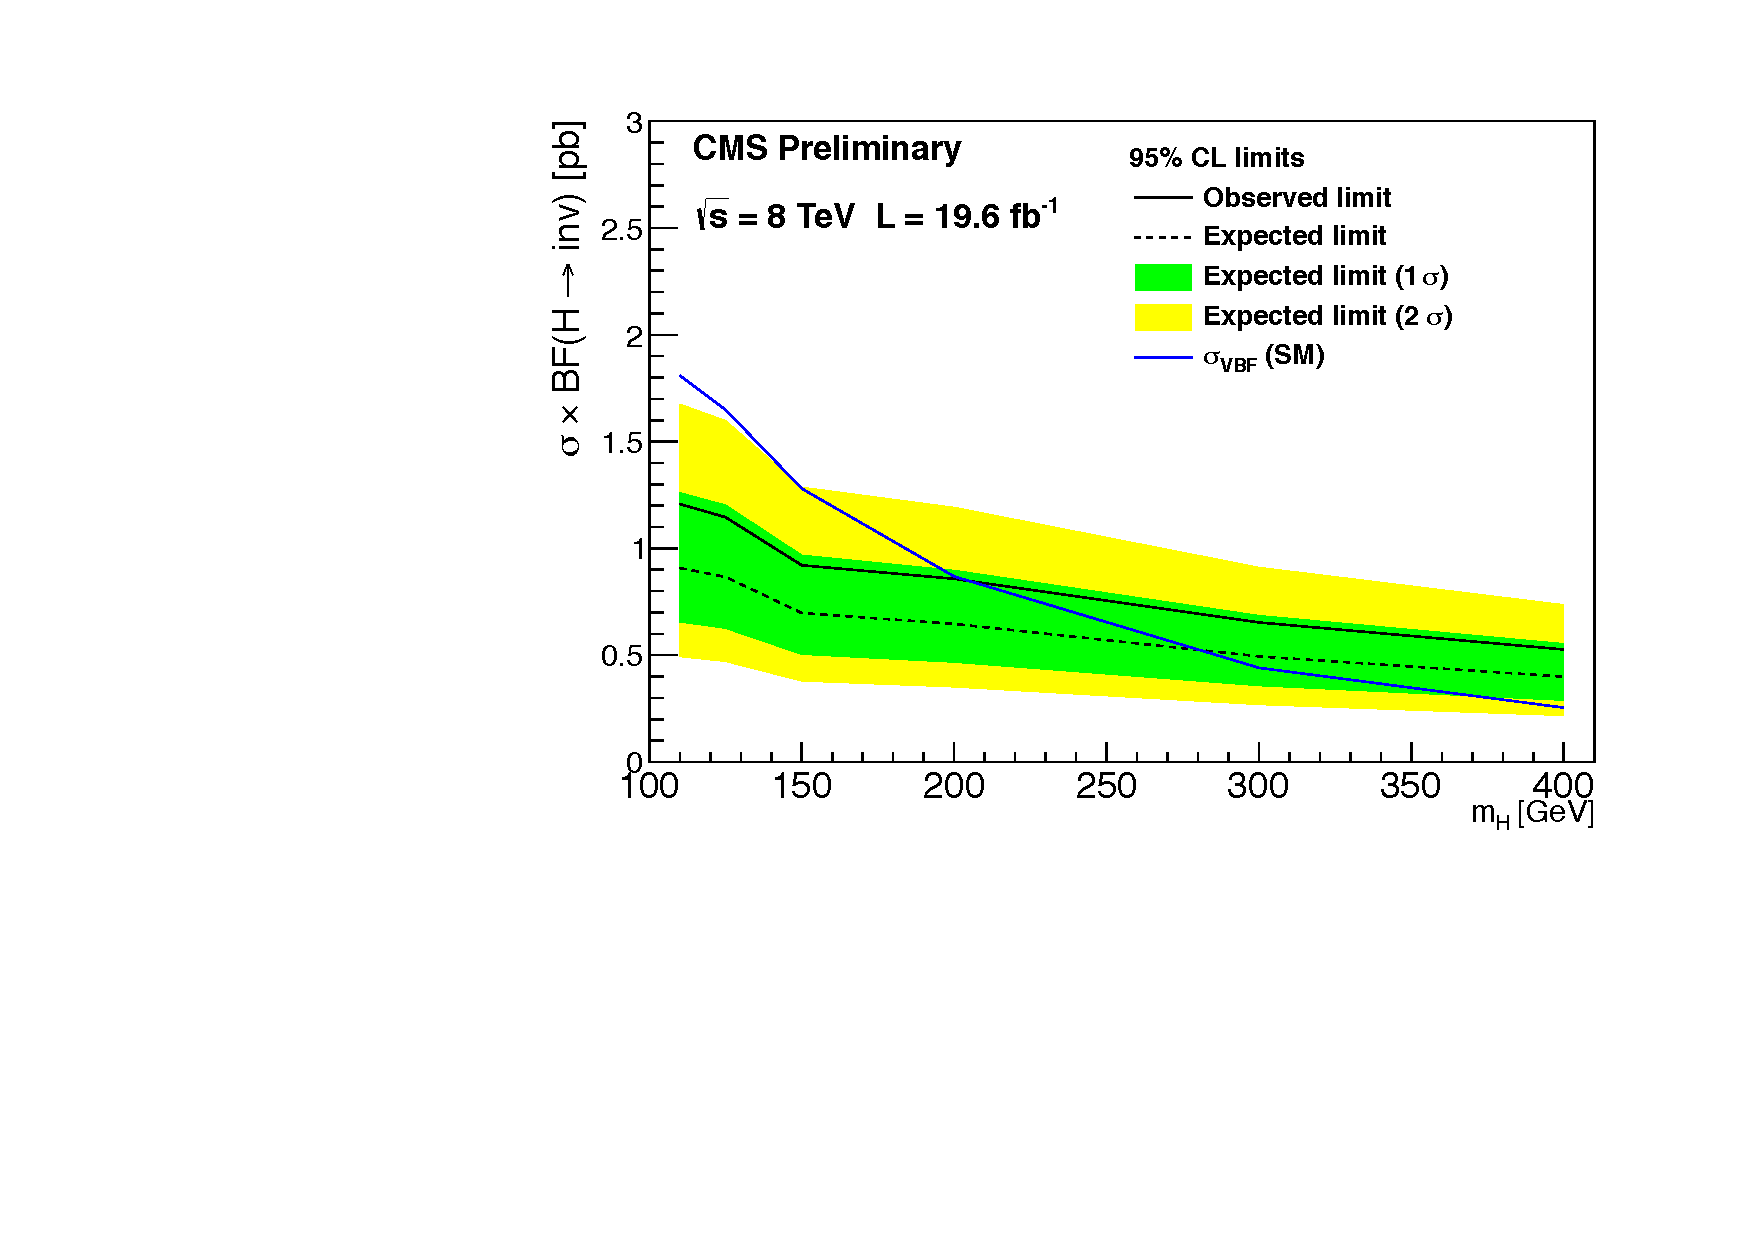
\includegraphics[width=\textwidth]{TalkPics/iccms091013/XSLimit.pdf}
    \column{.5\textwidth}
    \centering
    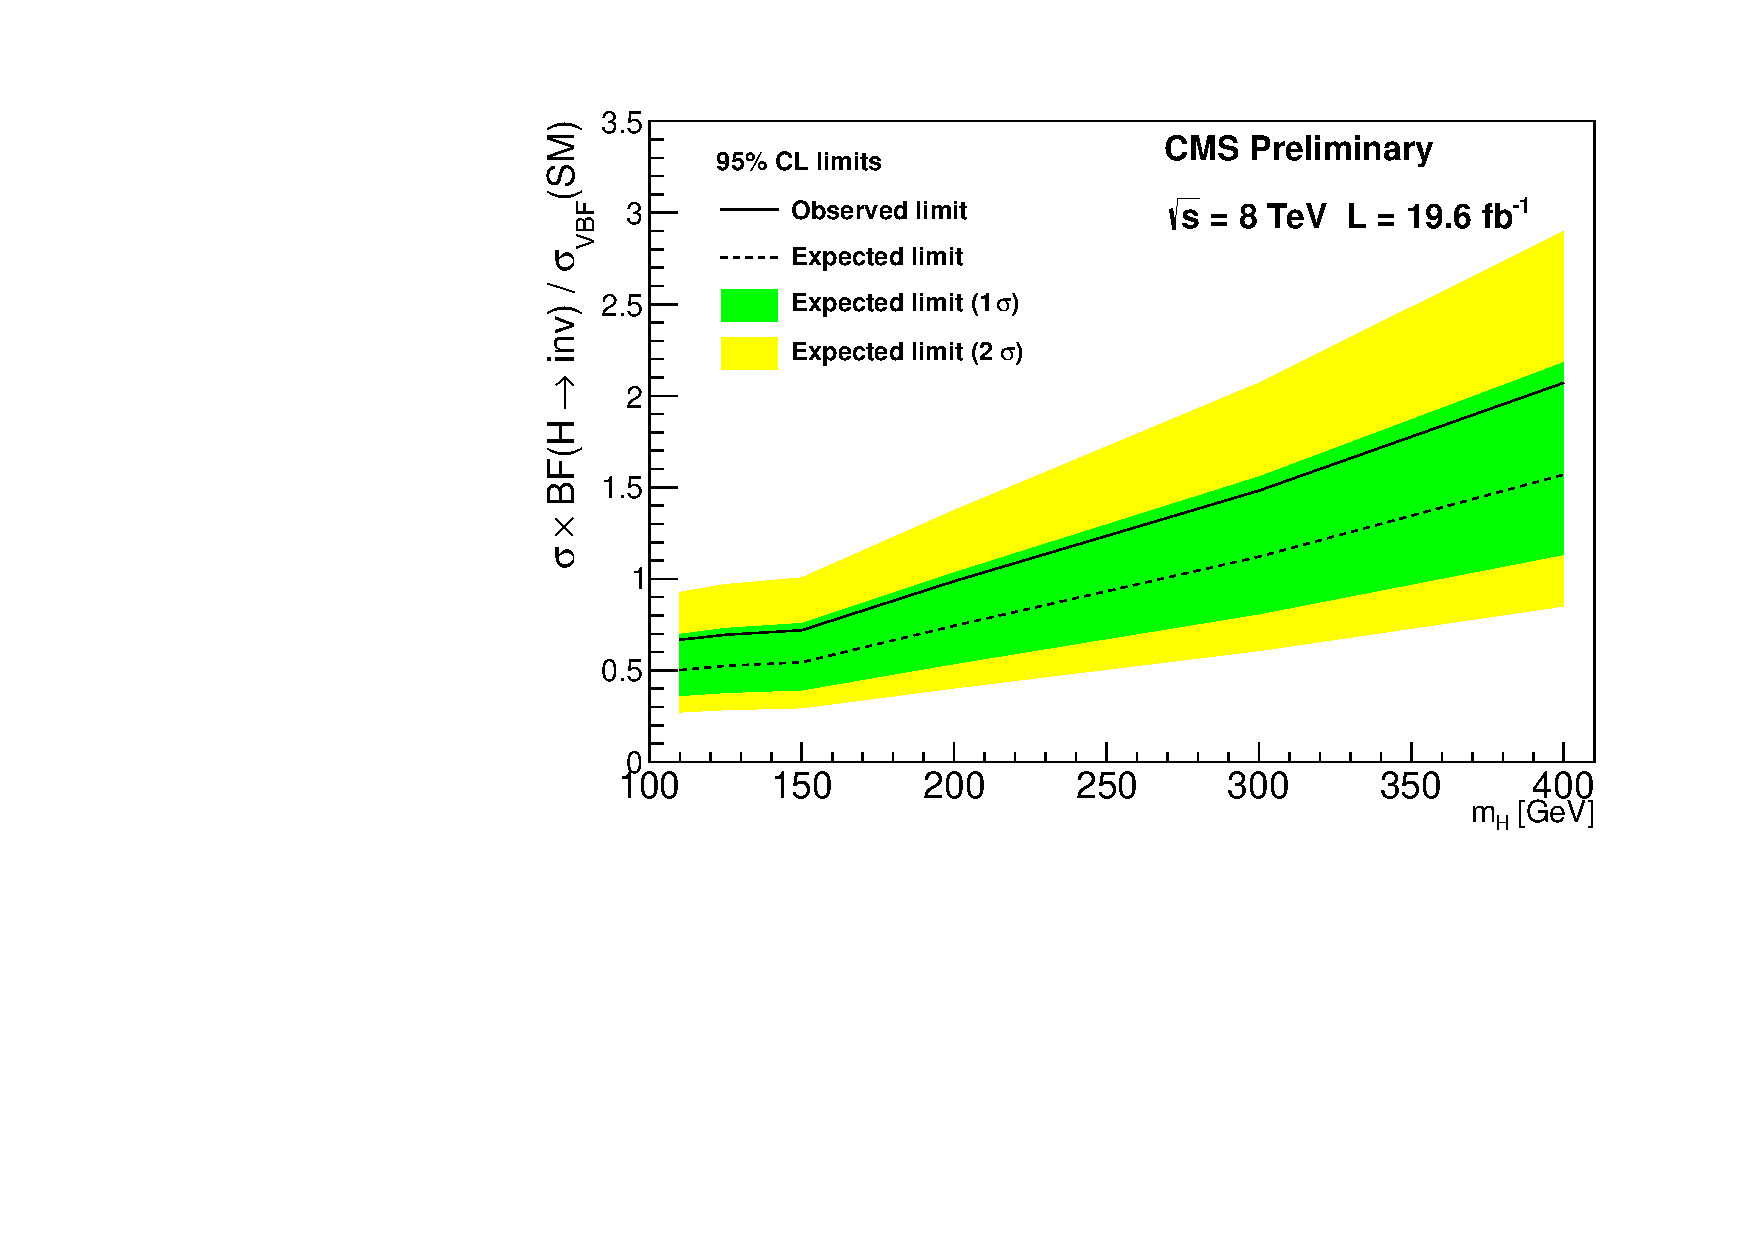
\includegraphics[width=\textwidth]{TalkPics/iccms091013/xsiLimit.pdf}
  \end{columns}
  \vspace{-0.2cm}
  \begin{block}{}
    \scriptsize
    \begin{itemize}
    \item Expected $339\pm36(stat.)\pm50(syst.)$ events, observed 390 events
    \item Limits produced with standard CMS Higgs combination package
    \item 95\% CL observed (expected) limit on the invisible BR for 125 GeV: 69(53)\%
    \end{itemize}
  \end{block}
\end{frame}

\begin{frame}
  \frametitle{ZH$\rightarrow$invisible}
  \begin{columns}
    \column{.5\textwidth}
    \begin{block}{\scriptsize Current ZH$\rightarrow$ invisible analyses}
      \scriptsize
    \begin{itemize}
    \item The Higgs to invisible analysis is also done in the ZH channel where the Z boson decays to two leptons (HIG-13-018)
    \item[-] 95\% CL observed (expected) limit on the invisible BR for 125 GeV: 75(91\%)
    \item A further analysis where the Z boson decays to two b quarks is in progress (HIG-13-028)
    \end{itemize}
    \end{block}
    
    \column{.5\textwidth}
    \vspace{.5cm}
    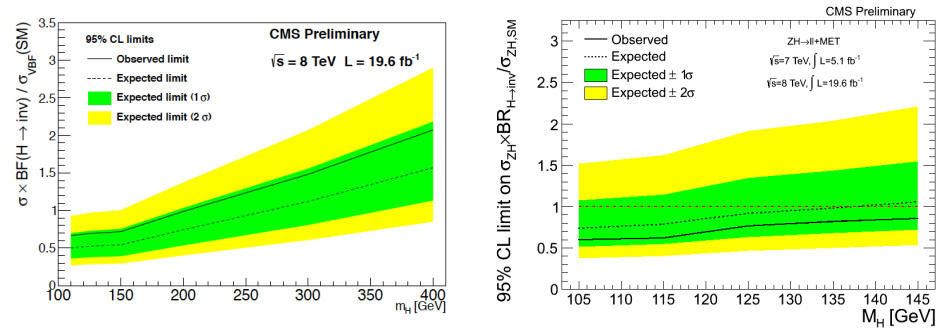
\includegraphics[clip=true,trim=400 0 0 0,width=\textwidth]{individualresults.png}  
  \end{columns}
\end{frame}

%!!CAN BE COVERED ABOVE

\begin{frame}
  \frametitle{Combining the ZH and VBF channels}
  \begin{block}{\scriptsize Datacards}
  \begin{itemize}
    \scriptsize
  \item VBF and ZH analysis have datacards at different Higgs boson mass points
  \item For the VBF channel only the signal yield is Higgs boson mass dependent
  \item[-] New datacards can therefore be made by interpolating the signal yields (details in backup)
  \end{itemize}
  \end{block}
  \begin{block}{\scriptsize Combination method}
    \scriptsize
    \begin{itemize}
    \item These new datacards were combined with the ZH cards using the standard Higgs group combination tool
    \item Luminosity uncertainties are considered correlated between analyses
    \item[-] All other uncertainties are considered to be uncorrelated (see discussion later)
    \end{itemize}
  \end{block}
\end{frame}

\begin{frame}
  \frametitle{Preliminary Results}
  \centering
  \vspace{-.13cm}
  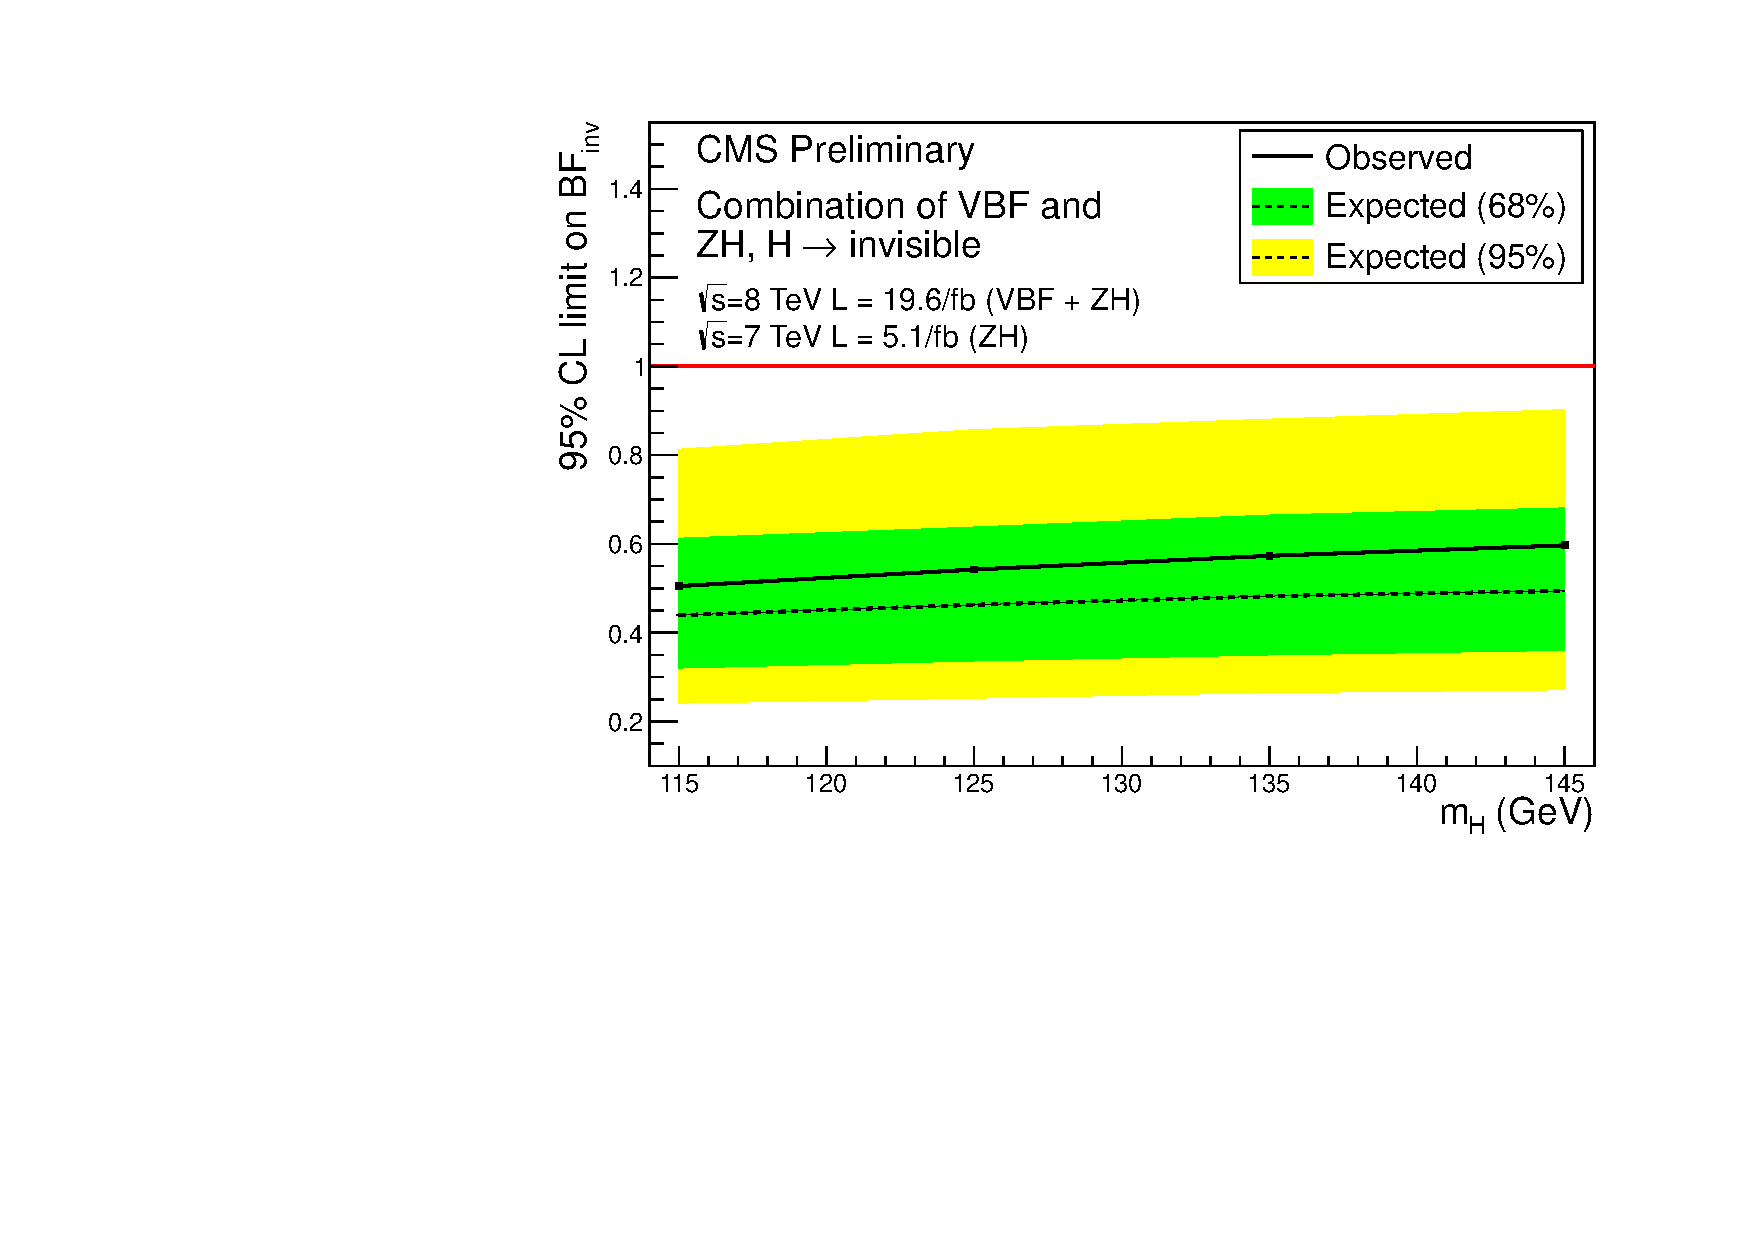
\includegraphics[clip=true,trim=0 5 0 35, width=.8\textwidth]{TalkPics/invlimitfinalfromPASs.pdf}
  \vspace{-.2cm}
  \begin{block}{}
  \begin{itemize}
  \item Observed (expected) limit at 125 GeV is 54(46)\%
  \item Made public through analysis twikis
  \end{itemize}
  \end{block}
\end{frame}

%!!INCORPORATE ELSEWHERE AND REMOVE

\begin{frame}
  \frametitle{Improvements for Paper}
  \begin{block}{\scriptsize Consideration of uncertainties}
    \scriptsize
    \begin{itemize}
    \item Current VBF channel datacards do not consider correlations between uncertainties
    \item[-] New datacards are being produced which separate out the uncertainty sources
    \item The following uncertainties will be considered correlated between the two channels
    \item[-] luminosity, jet energy scale and resolution, met scale, pdf uncertainties
    \end{itemize}
  \end{block}
  \begin{block}{\scriptsize W$\rightarrow\tau\nu$ background}
    \scriptsize
      \begin{itemize}
      \item Disagreement seen between IC cross-check and main analysis
      \item[-] Disagreement found to be from different jet smearing methods
      \item[-] Work is being done to synchronise these methods
      \end{itemize}
  \end{block}
\end{frame}

%!!UPDATE

\begin{frame}
  \frametitle{Summary}
  \begin{block}{\footnotesize Current Status}
    \footnotesize
  \begin{itemize}
  \item A limit has been placed on the invisible branching fraction of the Higgs boson produced in the VBF channel:
  \item[-] Observed(Expected) limit at 95\% CL is 69(53)\% for a 125 GeV Higgs
  \item This result has been combined with the ZH$\rightarrow$ll+invisible channel
  \item[-] Observed(Expected) limit at 95\% CL is 54(46)\% for a 125 GeV Higgs
  \item This combined result is the current strongest limit on BR(invisible)
  \end{itemize}
  \end{block}
  \begin{block}{\footnotesize Plans}
    \footnotesize
  \begin{itemize}
  \item A paper for the prompt data is being written with the improvements discussed above
  \item An improved analysis is planned using the parked data
  \end{itemize}
  \end{block}
\end{frame}

%!!CHANGE TO FUTURE

\begin{frame}\label{lastframe}
  \frametitle{Parked Data}
  \begin{block}{}
    \begin{itemize} 
    \item{\color{red} IC pushed strongly for data parking}    
    \item Jet $E_{T}>35(30) GeV$, $\Delta\eta_{jj}>3.5$, $m_{jj}>700 GeV$
    \item[-] Trigger with $E_{T}>30 GeV$ added for run D
    \item Good efficiency for visible and invisible VBF Higgs channels
    \item Plan to update result with parked data included after paper
    \end{itemize}
  \end{block}
\end{frame}

\begin{frame}%!! UPDATE ALL BACKUP
  \frametitle{BACKUP}
\end{frame}

%OBJECTS
\begin{frame}
  \frametitle{Objects}
  \begin{columns}
    \column{.5\textwidth}
    \begin{block}{\scriptsize VBF Selections}
      \scriptsize
      \begin{itemize}
      \item \color{red} Applied to all regions
      \item 2 jets:
      \item[-] Both jets must pass loose PUJetID
      \item[-] $p_{T} > 50 GeV$,  $|\eta| < 4.7$
      \item[-] $|\Delta\eta|>4.2$ , $\eta_{j_{1}}*\eta_{j{_2}}<0$
      \item[-] $m_{jj} > 1100 GeV$
      \end{itemize}
    \end{block}
    \begin{block}{\scriptsize MET}
      \scriptsize
      \begin{itemize}
      \item Using Type 0 + 1 Corrections
      \end{itemize}
    \end{block}
    \column{.5\textwidth}
    \begin{block}{\scriptsize Electrons}
      \scriptsize
      \begin{itemize}
        \item Veto:
        \item[-] $p_{T}>10 GeV$, $|\eta<2.5|$
        \item[-] rel PF Iso $< 0.2$
        \item Tight:
        \item[-] $p_{T}>20 GeV$, $|\eta<2.5|$
      \end{itemize}
    \end{block}
    \begin{block}{\scriptsize Muons}
      \scriptsize
      \begin{itemize}
        \item Veto:
        \item[-] $p_{T}>10 GeV$, $|\eta<2.1|$
        \item[-] rel PF Iso $< 0.2$
        \item Tight: 
        \item[-] $p_{T}>20 GeV$, $|\eta<2.1|$
      \end{itemize}
    \end{block}
  \end{columns}
\end{frame}

\begin{frame}
  \frametitle{Signal Yield interpolation}
  \begin{columns}
    \column{.5\textwidth}
    \begin{itemize}
    \item $N_{Signal}=eff. \times acc. \times \mathcal L\sigma$
    \item Luminosity is constant
    \item Yield over cross-section is thus proportional to efficiency times acceptance
    \item Signal yields were produced at 115, 125(to cross-check), 135 and 145 GeV for the VBF channel
    \item[-] Cross-sections from LHC-HXSWG were used
    \end{itemize}
    \column{.5\textwidth}
    \centering
    \hspace{-.5cm}
    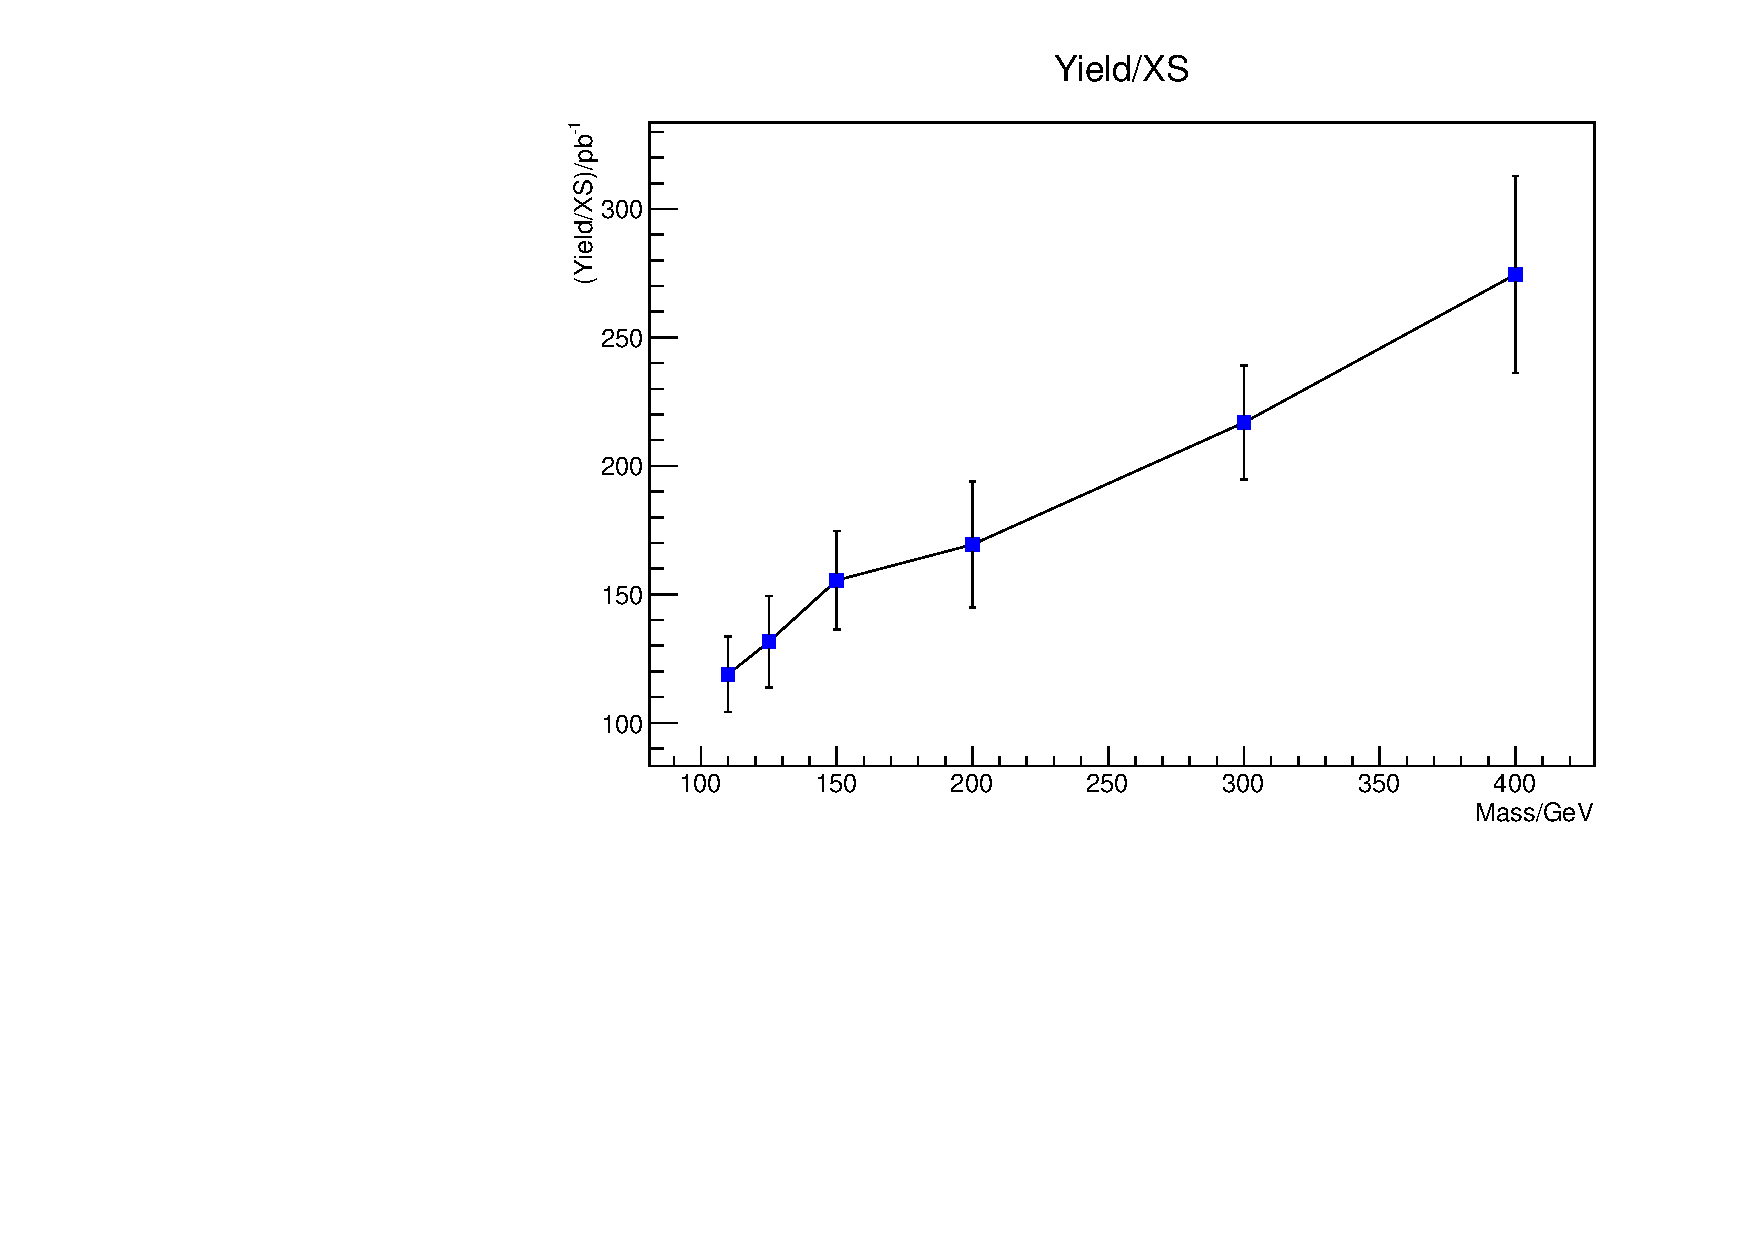
\includegraphics[clip=true,trim=0 0 0 30, width=1.2\textwidth]{yieldoverxs.pdf}
  \end{columns}
\end{frame}

\begin{frame}
  \frametitle{$W$+jets background $m_{T}$ plots}
  \begin{columns}
    \column{.33\textwidth}
    $e\nu$
    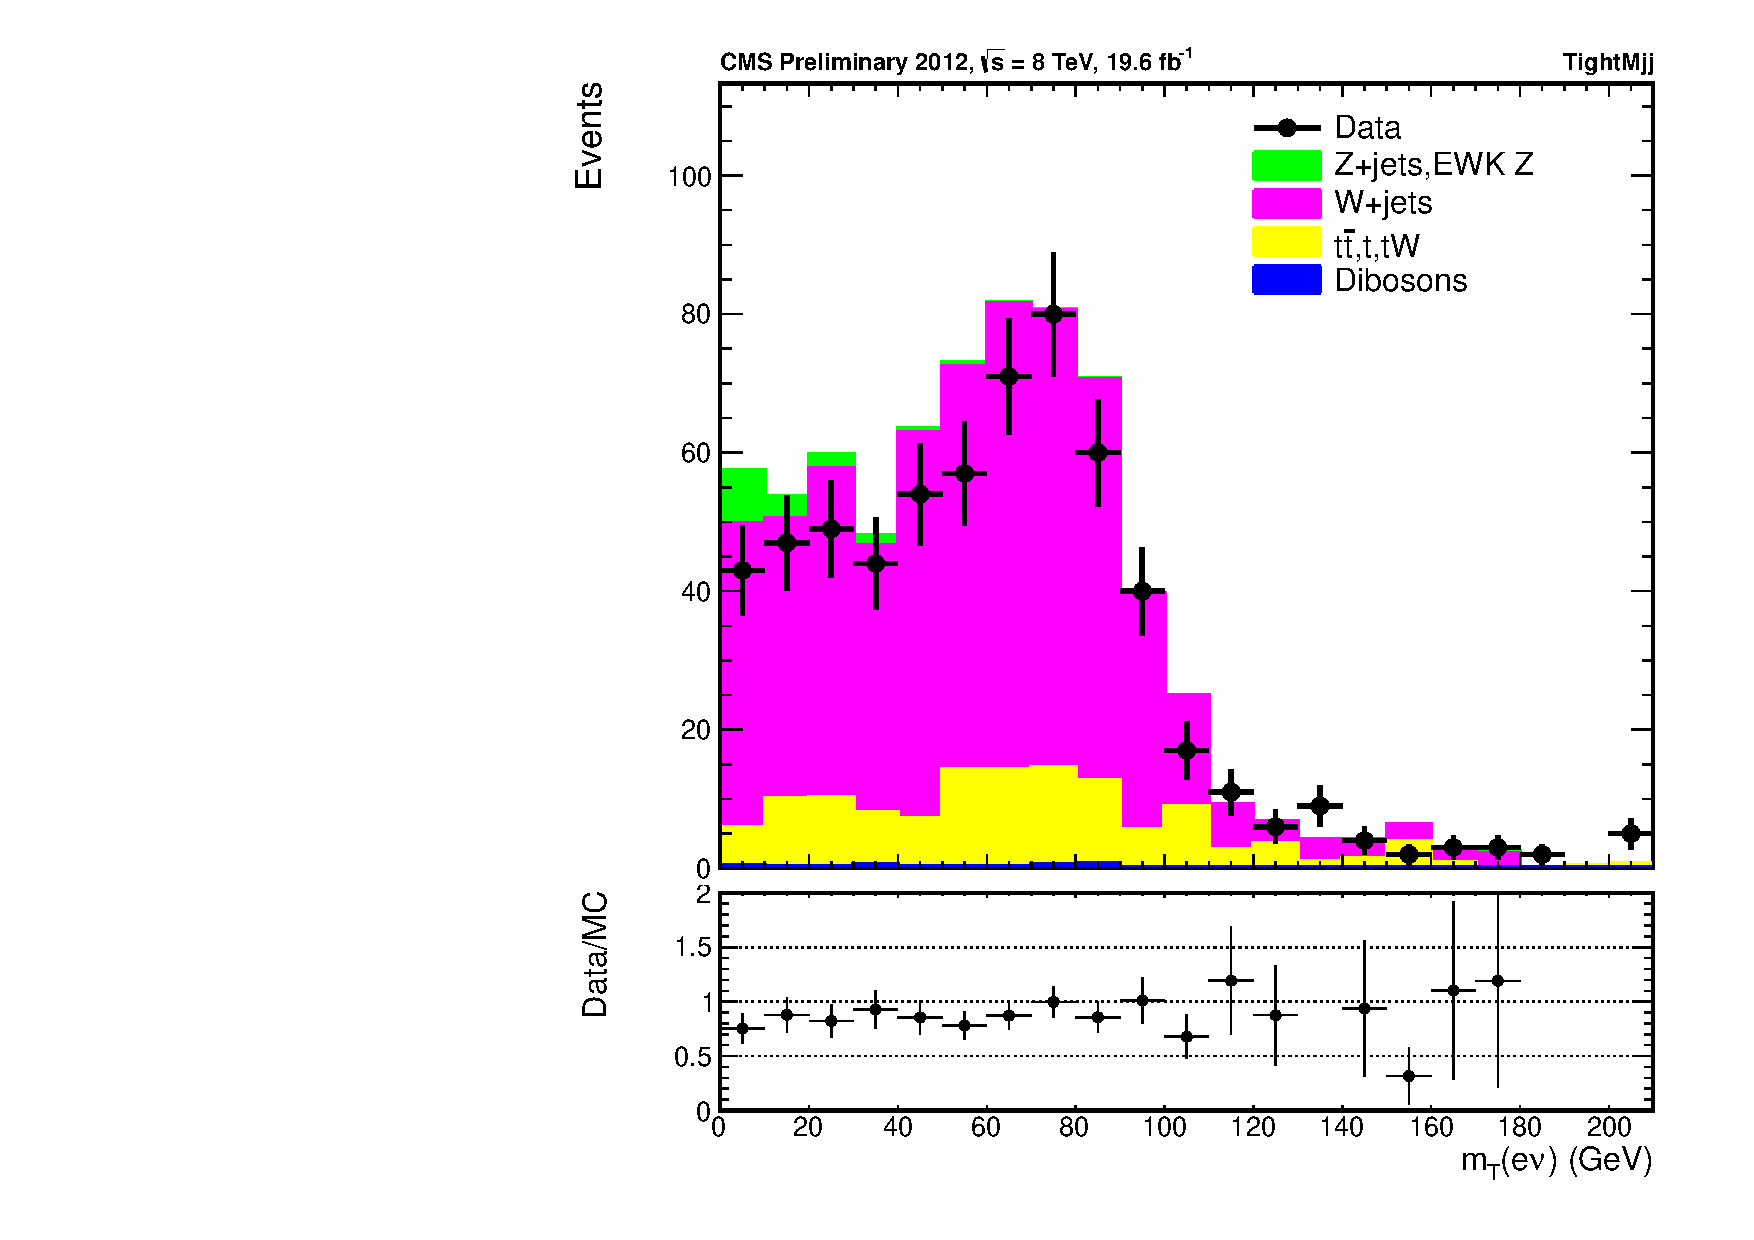
\includegraphics[width=\textwidth]{TalkPics/mt_enu_TightMjj.pdf}
    \column{.33\textwidth}
    $\mu\nu$
    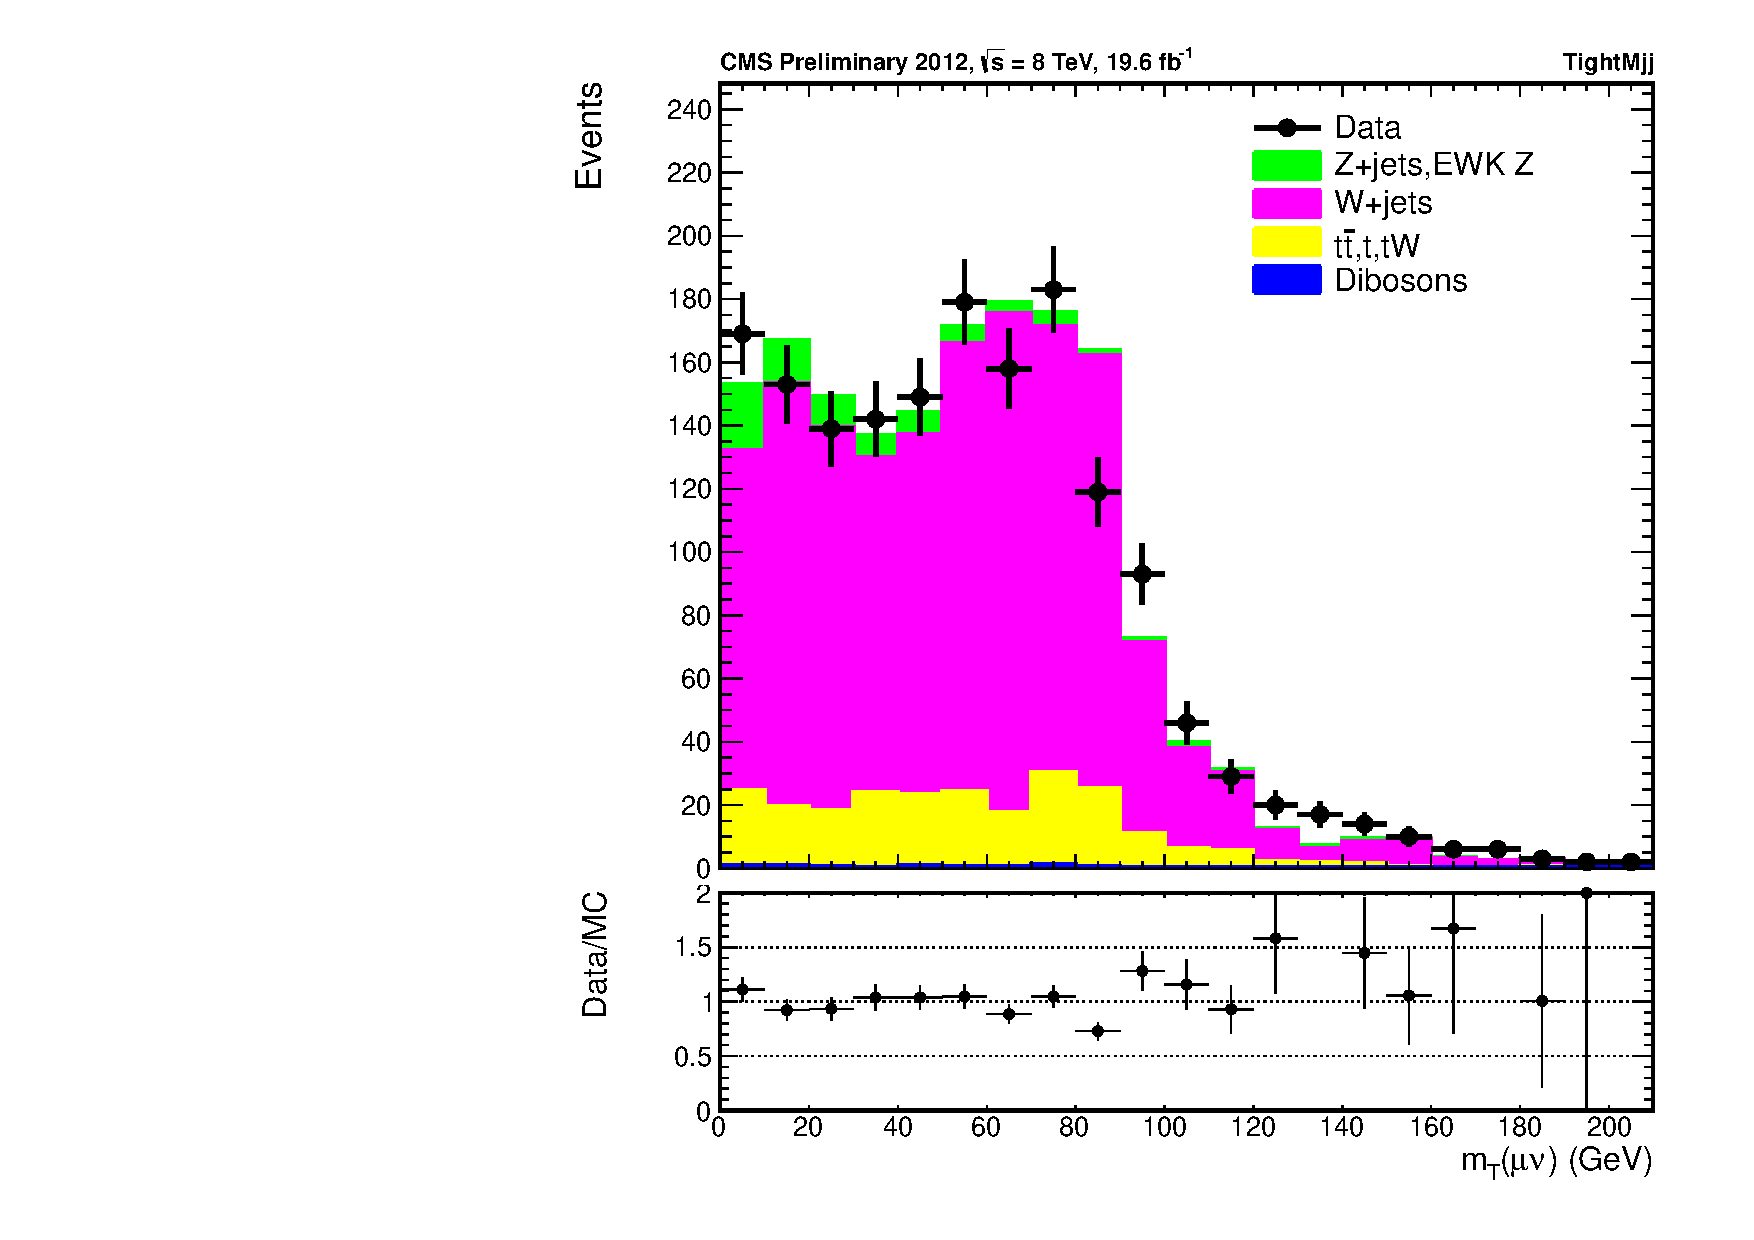
\includegraphics[width=\textwidth]{TalkPics/mt_munu_TightMjj.pdf}
    \column{.33\textwidth}
    $\tau\nu$
    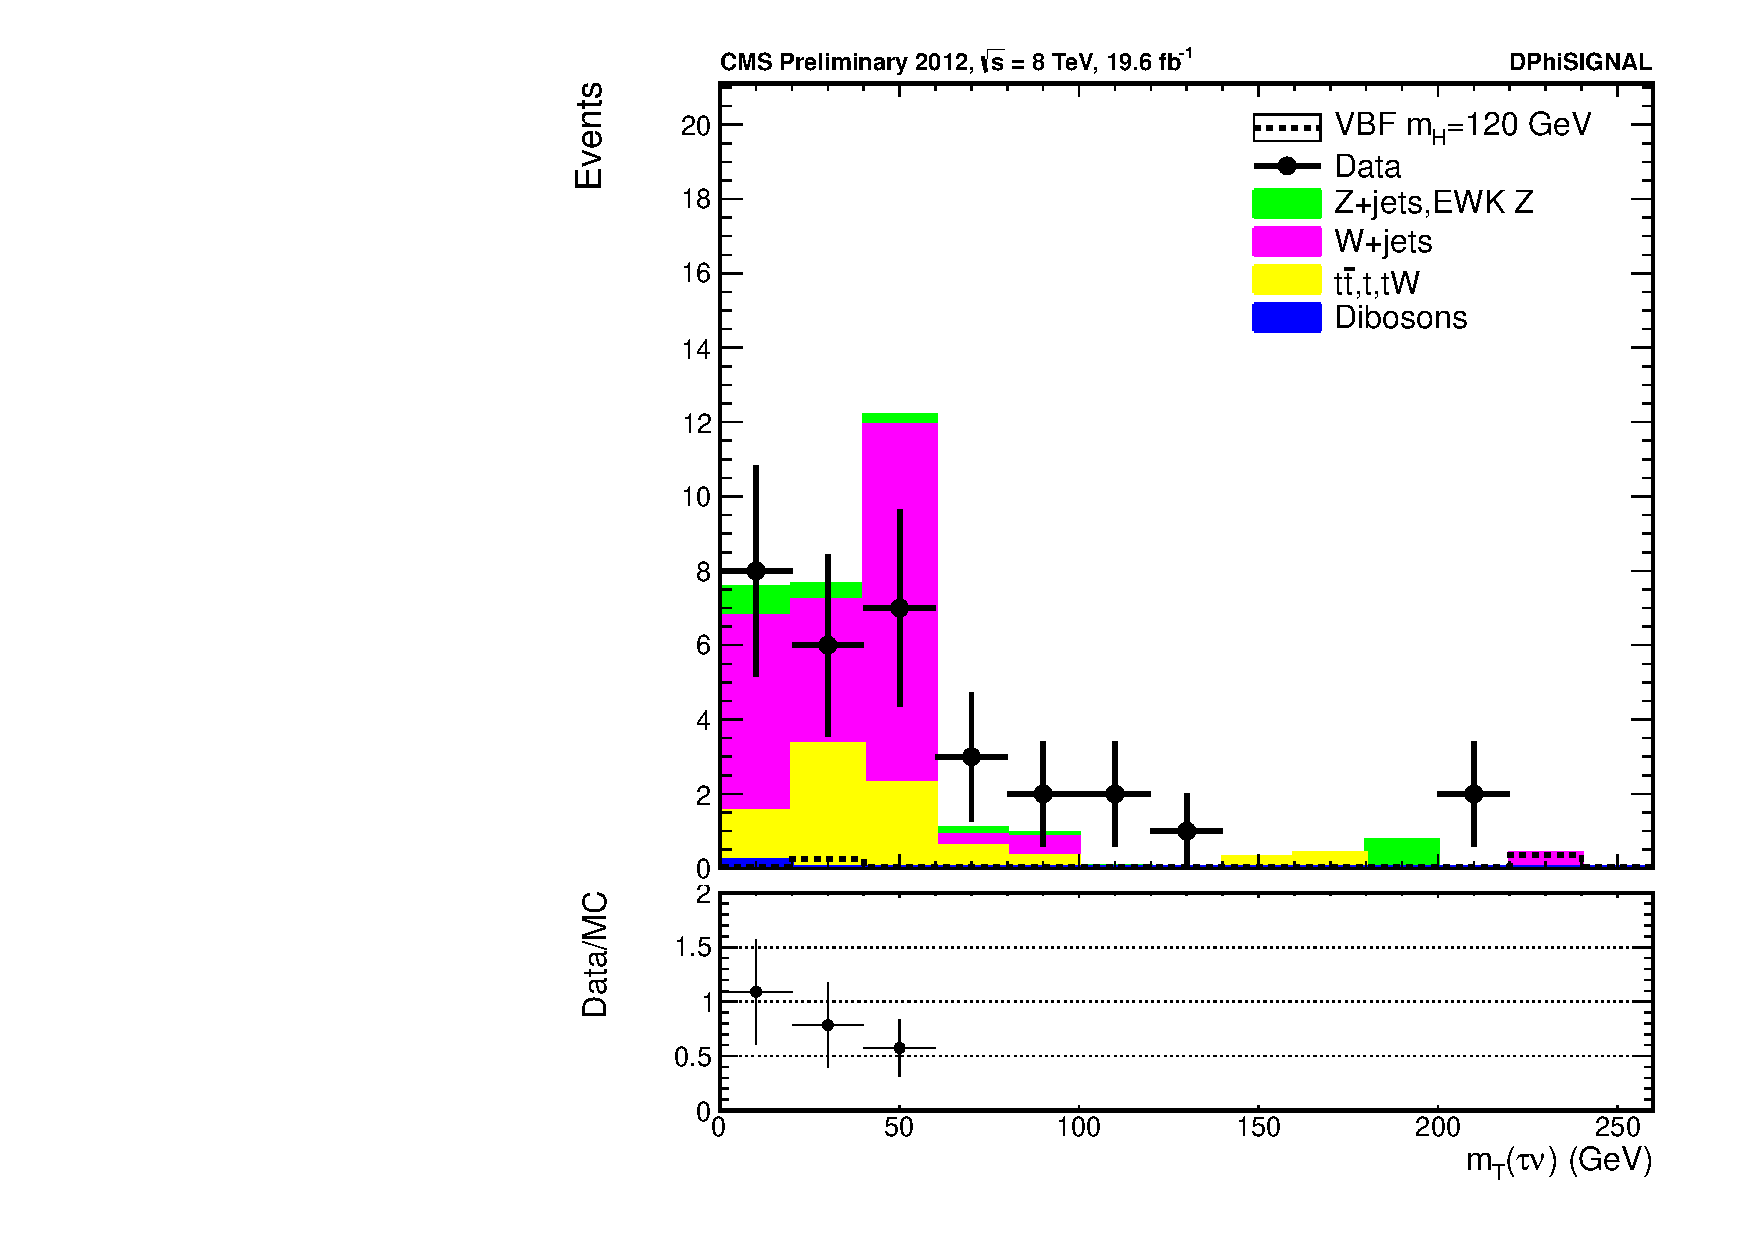
\includegraphics[width=\textwidth]{TalkPics/mt_taunu_2012_DPhiSIGNAL.pdf}
  \end{columns}
\end{frame}
\end{fmffile}
\end{document}
